% %%%%%%%%%%%%%%%%%%%%%%%%%%%%%%%%%%%%%%%%%%%%%%%%%%%%%%%%%%%%%%%%%%%%%%%%%%%%%
% thesis.tex: Primary TeX control file for thesis.
% %%%%%%%%%%%%%%%%%%%%%%%%%%%%%%%%%%%%%%%%%%%%%%%%%%%%%%%%%%%%%%%%%%%%%%%%%%%%%
\documentclass[11pt, oneside]{mnthesis}
\usepackage{epsfig} % Allows the inclusion of eps files
\usepackage{epic} % Enhanced picture mode
\usepackage{eepic} % Extensions for epic
\usepackage{units} % SI unit typesetting
\usepackage{url} % URL handling
\usepackage{longtable} % Tables that continue onto multiple pages
\usepackage{mathrsfs} % Support for \mathscr script
\usepackage{multirow} % Span rows in tables
%\usepackage{bigstrut} % Space struts in tables up and down
\usepackage{amssymb} % AMS math symbols and helpers
\usepackage{graphicx} % Enhanced graphics support
\usepackage{setspace} % Adjust spacing in captions, single by default
\usepackage{xspace} % Automatically adjusting space after macros
\usepackage{amsmath} % \text, and other math formatting options
\usepackage{siunitx} % \num{} formatting and SI unit formatting
\usepackage{booktabs} % Enhanced tables with \toprule, etc.
\usepackage{hyperref} % Add clickable links to other parts of the document
\usepackage[noabbrev,capitalize]{cleveref} % Automatically determine \cref type

\usepackage[hang,flushmargin]{footmisc} % Prevent indent in footnotes. 

% Put captions tighter to their figures. Not clear if it actually works. 
\setlength{\abovecaptionskip}{0pt}

\usepackage{xcolor} % so we can put todo notes in color. 

\usepackage{doi} % Link to doi in the bibliography. Doesn't seem to work. 

\usepackage{parskip} % http://ctan.org/pkg/parskip vskip instead of indent. 

\usepackage{float} % Sometimes you want to tell LaTeX to put an image RIGHT HERE. 


% Configure the siunitx package
\sisetup{
    group-separator = {,}, % Use , to separate groups of digits, like 12,345
    list-final-separator = {, and } % Always use the serial comma in \SIlist
}

% Configure the cleveref package
\newcommand{\creflastconjunction}{, and } % Always use the serial comma




% Names with special characters. 
\newcommand{\Alfven}{Alfv\'en\xspace}
\newcommand{\Ampere}{Amp\`ere\xspace}

% To make sure the capitalization is consistent. 
\newcommand{\ohmlaw}{Ohm's Law\xspace}
\newcommand{\amplaw}{\Ampere's Law\xspace}
\newcommand{\farlaw}{Faraday's Law\xspace}

% Field-aligned unit vectors. 
\newcommand{\xhat}{\ensuremath{\hat{x}}\xspace}
\newcommand{\yhat}{\ensuremath{\hat{y}}\xspace}
\newcommand{\zhat}{\ensuremath{\hat{z}}\xspace}

% Spherical unit vectors. 
\newcommand{\rhat}{\ensuremath{\hat{r}}\xspace}
\newcommand{\qhat}{\ensuremath{\hat{\theta}}\xspace}
\newcommand{\fhat}{\ensuremath{\hat{\phi}}\xspace}

% Use underlines for vectors and tensors. 
\renewcommand{\vec}[1]{\underline{#1}}
\newcommand{\tensor}[1]{\underline{\underline{#1}}}

% Differential operators. 
\newcommand{\dd}[1]{\ensuremath{ \frac{\partial}{\partial #1} }\xspace}
\newcommand{\ddt}{\dd{t}\xspace}
\newcommand{\curl}[1]{\ensuremath{ \nabla \times \vec{#1} }\xspace}
\renewcommand{\div}[1]{\ensuremath{ \nabla \cdot \vec{#1} }\xspace}
\newcommand{\grad}[1]{\ensuremath{ \nabla #1 }\xspace}

% Properly-scaled parentheses for grouping terms or for arguments. 
\newcommand{\lr}[1]{ \left( #1 \right) }
\newcommand{\lrsmall}[1]{ \left( {\scriptstyle #1} \right) }
\renewcommand{\arg}[1]{\!\lr{#1}}
\newcommand{\argsmall}[1]{\!\lrsmall{#1}}
\newcommand{\lrb}[1]{ \left[ #1 \right] }

% Circled plus-minus symbol. Solving quartics requires \pm and \opm. 
\newcommand{\opm}{ \text{ \textcircled{ \ensuremath{\hskip -0.2em \pm} } } \xspace}

% Define a better looking eV by moving the V slightly left
\DeclareSIUnit\electronvolt{e\hspace{-0.08em}V}

\DeclareSIUnit\RE{R_E}


\newcommand{\dt}{\ensuremath{\delta \hspace{-0.1em} t} \xspace}



% Azimuthal modenumber, typically indicated with a lowercase m. 
\newcommand{\azm}{\ensuremath{m_{azimuthal}}\xspace}

% Azimuthal modenumber, typically indicated with a lowercase m. 
\newcommand{\me}{\ensuremath{m_{e}}\xspace}

% Jacobian dererminant, typically indicated with a capital J, which we are using for current. 
\newcommand{\jac}{\ensuremath{D}\xspace}

% Dispersion tensor, typically indicated with... a capital D?
\newcommand{\dispersiontensor}{\tensor{T}\xspace}


% These things just get used a lot in the dispersion relation chapter...

% Boris-corrected speed of light. 
\newcommand{\cb}{\ensuremath{c_B} \xspace}

% Boris-corrected plasma frequency. 
\newcommand{\ob}{\ensuremath{\omega_B} \xspace}

% Boris-corrected electric constant. 
\newcommand{\eb}{\ensuremath{\epsilon_B} \xspace}

% Alfven speed. 
\newcommand{\va}{\ensuremath{v_A} \xspace}

% Perpendicular electric constant. 
\newcommand{\ep}{\ensuremath{\epsilon_\bot} \xspace}

% Epsilon zero. 
\newcommand{\ez}{\ensuremath{\epsilon_0} \xspace}

% Conductivities. 
\newcommand{\sz}{\ensuremath{\sigma_0} \xspace}
\newcommand{\sh}{\ensuremath{\sigma_H} \xspace}
\renewcommand{\sp}{\ensuremath{\sigma_P} \xspace}




\newcommand{\spe}{\ensuremath{\frac{\sigma_P}{\ep}} \xspace}
\newcommand{\she}{\ensuremath{\frac{\sigma_H}{\ep}} \xspace}




% 3x3 matrix. 
\newcommand{\mmm}[9]{ \left[ \begin{array}{ccc}
    #1 & #2 & #3 \\
    #4 & #5 & #6 \\
    #7 & #8 & #9
  \end{array} \right] }

% 2x2 matrix. 
\newcommand{\mm}[4]{ \left[ \begin{array}{cc}
    #1 & #2 \\
    #3 & #4
  \end{array} \right] }

% 2x1 matrix, or 2-vector. 
\newcommand{\vv}[2]{ \left[ \begin{array}{c}
    #1 \\
    #2
  \end{array} \right] }


% Physics constants
\newcommand{\C}{{\mathrm{c}}}

% Add space between rows of tables
\newcommand{\spacerows}[1]{\renewcommand{\arraystretch}{#1}}









\linespread{1.3}

% Compile only the chapters listed here. This may make the compile faster, but
% it's not necessary. 
%\includeonly{
%    preliminaries/title,
%    chapters/intro,
%    chapters/model,
%    chapters/math,
%    chapters/results,
%    chapters/data,
%    chapters/conclusion,
%    chapters/app_geometry,
%    chapters/app_integrating,
%}



% %%%%%%%%%%%%%%%%%%%%%%%%%%%%%%%%%%%%%%%%%%%%%%%%%%%%%%%%%%%%%%%%%%%%%%%%%%%%%
% %%%%%%%%%%%%%%%%%%%%%%%%%%%%%%%%%%%%%%%%%%%%%%%%%%%%%%% Mark this as a draft. 
% %%%%%%%%%%%%%%%%%%%%%%%%%%%%%%%%%%%%%%%%%%%%%%%%%%%%%%%%%%%%%%%%%%%%%%%%%%%%%
\draft
% %%%%%%%%%%%%%%%%%%%%%%%%%%%%%%%%%%%%%%%%%%%%%%%%%%%%%%%%%%%%%%%%%%%%%%%%%%%%%
% %%%%%%%%%%%%%%%%%%%%%%%%%%%%%%%%%%%%%%%%%%%%%%%%%%%%%%%%%%%%%%%%%%%%%%%%%%%%%
% %%%%%%%%%%%%%%%%%%%%%%%%%%%%%%%%%%%%%%%%%%%%%%%%%%%%%%%%%%%%%%%%%%%%%%%%%%%%%



\begin{document}
%\bibliographystyle{hunsrt} % Default bibliography style file moved to archive/
\bibliographystyle{abbrv}

% Title and other sections that come before the body of the document
%%%%%%%%%%%%%%%%%%%%%%%%%%%%%%%%%%%%%%%%%%%%%%%%%%%%%%%%%%%%%%%%%%%%%%%%%%%%%%%%
% title.tex - Set up the beginning of thesis.
%%%%%%%%%%%%%%%%%%%%%%%%%%%%%%%%%%%%%%%%%%%%%%%%%%%%%%%%%%%%%%%%%%%%%%%%%%%%%%%%

% Uncomment to turn on draft mode, which changes the title page to have a draft
% label and date of compilation
%\draft

% Set the type of thesis
\phd % use if for a Ph.D. dissertation
%\ms % use if for a Master of Science thesis

% Set the title and your name. Remember that the guidelines state:
%
% "The title of the thesis must not contain chemical or mathematical formulas,
% symbols, superscripts, subscripts, Greek letters, or other non-standard
% characters; words must be substituted."
\title{\bf Modeling Current-Driven Pc4 Pulsations in Two and a Half Dimensions}
\author{Charles A McEachern}
% Advisor name, put co-advisors here as well separated by commas
\director{Robert L Lysak}

% Specify the month and year; if commented out then these default to the
% current month and year
\submissionmonth{April}
\submissionyear{2016}

% Pages after the title page
\abstract{% %%%%%%%%%%%%%%%%%%%%%%%%%%%%%%%%%%%%%%%%%%%%%%%%%%%%%%%%%%%%%%%%%%%%%%%%%%%%%
% %%%%%%%%%%%%%%%%%%%%%%%%%%%%%%%%%%%%%%%%%%%%%%%%%%%%%%%%%%%%%%%%%%%% Abstract
% %%%%%%%%%%%%%%%%%%%%%%%%%%%%%%%%%%%%%%%%%%%%%%%%%%%%%%%%%%%%%%%%%%%%%%%%%%%%%

Abstract placeholder. 
}
\copyrightpage % Do you want copyright protection?
\acknowledgements{%%%%%%%%%%%%%%%%%%%%%%%%%%%%%%%%%%%%%%%%%%%%%%%%%%%%%%%%%%%%%%%%%%%%%%%%%%%%%%%%
% acknowledge.tex: Acknowledgements
%%%%%%%%%%%%%%%%%%%%%%%%%%%%%%%%%%%%%%%%%%%%%%%%%%%%%%%%%%%%%%%%%%%%%%%%%%%%%%%%

There are many people that have earned my gratitude for their contribution to my
time in graduate school.

%%%%%%%%%%%%%%%%%%%%%%%%%%%%%%%%%%%%%%%%%%%%%%%%%%%%%%%%%%%%%%%%%%%%%%%%%%%%%%%%
}
\dedication{% %%%%%%%%%%%%%%%%%%%%%%%%%%%%%%%%%%%%%%%%%%%%%%%%%%%%%%%%%%%%%%%%%%%%%%%%%%%%%
% %%%%%%%%%%%%%%%%%%%%%%%%%%%%%%%%%%%%%%%%%%%%%%%%%%%%%%%%%%%%%%%%%% Dedication
% %%%%%%%%%%%%%%%%%%%%%%%%%%%%%%%%%%%%%%%%%%%%%%%%%%%%%%%%%%%%%%%%%%%%%%%%%%%%%

\todo{$\cdots$}

}

% Use a special preface
%\extra{\input{preface}}

% The \beforepreface command actually causes insertion of the title,
% abstract, signature, and copyright pages into the new document.
\beforepreface

% Define the text to go before the table of contents
\figurespage
\tablespage

% The \afterpreface command actually causes insertion of the
% contents, list of figures, etc. into the new document.
\afterpreface
%%%%%%%%%%%%%%%%%%%%%%%%%%%%%%%%%%%%%%%%%%%%%%%%%%%%%%%%%%%%%%%%%%%%%%%%%%%%%%%%


% %%%%%%%%%%%%%%%%%%%%%%%%%%%%%%%%%%%%%%%%%%%%%%%%%%%%%%%%%%%%%%%%%%%%%%%%%%%%%
% %%%%%%%%%%%%%%%%%%%%%%%%%%%%%%%%%%%%%%%%%%%%%%%%%%%%%%%%%%%%%%%%%%%%%%%%%%%%%
% %%%%%%%%%%%%%%%%%%%%%%%%%%%%%%%%%%%%%%%%%%%%%%%%%%%%%%%%%%%%%%%%%%%%%%%%%%%%%

\chapter{Introduction}
  \label{ch_intro}

\todo{In 1859, humanity was working hard to get its shit together.} The United States moved steadily toward the American Civil War, which would abolish slavery and consolidate the power of the federal government. A slew of conflicts in Southern Europe, such as the Austro-Sardinian War, set the stage for the unification of Italy. The Taiping Civil War -- one of the bloodiest conflicts of all time -- is considered by many to mark the beginning of modern Chinese history. Origin of Species was published. The first transatlantic telegraph cable was laid.

Meanwhile, ambivalent to humanity, the Sun belched an intense burst of charged particles and magnetic energy directly at Earth. The resulting geomagnetic storm\footnote{The Solar Storm of 1859 is also called the Carrington Event, after English astronomer Richard Carrington. He drew a connection between the storm's geomagnetic activity and the sunspots he had observed the day before.} caused telegraph systems to fail across the Western hemisphere\cite{green_2006}, electrocuting some operators. Displays of the northern lights were visible as far south as Cuba. 

The Solar Storm of 1859 was perhaps the most powerful in recorded history, but by no means was it a one-time event. The Sun discharges hundreds of coronal mass ejections (CMEs) per year, of all sizes, in all directions. In fact, a comparably large CME narrowly missed Earth in 2012\cite{nasa_2012}. Had it not, it's estimated\cite{lloyds_2013} that it would have caused widespread, long-term electrical outages, with a damage toll on the order of \num{e9} dollars. 

The Sun's extreme -- and temperamental -- effect on Earth's magnetic environment makes a compelling case for the ongoing study of space weather. Such research has evolved over the past century from sunspot counts and compass readings to multi-satellite missions and supercomputer simulations. Modern methods have dramatically increased humanity's understanding of the relationship between the Sun and the Earth; however, significant uncertainty continues to surround geomagnetic storms, substorms, and the various energy transport mechanisms that make them up. 

The present work focuses in particular on the phenomenon of field line resonance: \Alfven waves bouncing between the northern and southern hemispheres. Such waves play an important part in the energization of magnetospheric particles, the transport of energy from high to low altitude, and the driving of currents at the top of the atmosphere. 

%\todo{The storm of 1859 presented compelling evidence that the Sun drives geomagnetic activity. In the decades that followed, a model took shape to describe the mechanisms of energy transfer between the Sun and the Earth. Based on auroral observations and data from ground-based magnetometers, Birkeland argued for the existence of a constant outflow of electrons and ions from the Sun -- the solar wind. The advent of high-frequency radio communication allowed Kennelly, Heaviside, and others to probe the electrical properties of the upper atmosphere. }

%\todo{The study of space weather was revolutionized by the development of sounding rockets and satellites in the mid twentieth century. This allowed direct observation of the structure of the near-Earth environment, including, crucially, the waves that carry energy through it. }

%\todo{Not least among these advances was the discovery of \Alfven waves. {\Alfven}ic aurora. Carry energy and particles. }

%The study of space weather revolves around the transfer of energy from the Sun to the Earth. Ultra low frequency waves in particular are an important energy transport mechanism between the magnetosphere's outer boundary (at the solar wind) and its inner boundary (at the top of the atmosphere). 

%\footnote{Uppercase \X, \Y, and \Z are used to indicate GSE coordinates: \Xhat points from the Earth to the Sun; \Yhat is perpendicular to \Xhat in the Sun's ecliptic plane, pointing duskwards; \Zhat points north, out of the ecliptic plane. In later chapters, lowercase \x, \y, and \z are used to define a more-or-less analogous corodinate system with respect to Earth. }

% The moon is at \SI{60}{\RE}. 


  % =============================================================================
% =============================================================================
% =============================================================================
\section{The Near-Earth Environment}
  \label{sec_environment}


From Earth's surface to about \SI{100}{\km}, the atmosphere is a well-behaved fluid: a collisional ensemble of neutral atoms. However, beyond there, its behavior changes dramatically. As altitude increases, solar ultraviolet radiation becomes more intense, which ionizes atmospheric atoms. Density also decreases, slowing collisional recombination. Whereas the neutral atmosphere is held against Earth's surface by gravity, the behavior of charged particles is dominated by Earth's geomagnetic field... and the electromagnetic disturbances created as that field is hammered by the solar wind. 

\todo{Neutral density is larger than charged particle density (?) but it doesn't matter because mean free path is huge. }

The present section outlines the structure of the magnetosphere; that is, the region of space governed primarily by Earth's magnetic field. Particular emphasis is placed on structures which relate closely to field line resonance. 

% -----------------------------------------------------------------------------
% -----------------------------------------------------------------------------
% -----------------------------------------------------------------------------
\subsection{The Outer Magnetosphere}

During quiet times\footnote{Geomagnetically active times are the topic of \cref{sec_storms}}, the behavior of the magnetosphere is driven by the solar wind: a hot, rarefied, fast-moving solar outflow threaded by the Sun's magnetic field\footnote{Usual solar wind velocities, densities, and temperatures fall on the order of \SI{100}{\km/\s}, \SI{10}{\percc}, and \SI{1}{\keV} respectively. At Earth's orbit, the Sun's magnetic field has a magnitude around \SI{1}{\nT}. }. 

The magnetosphere's outer boundary represents a balance between the solar wind dynamic pressure and the magnetic pressure of Earth's dipole field. On the dayside, the dipole is compressed, pushing the magnetopause to within \SI{10}{\RE}\footnote{Distances in the magnetosphere are typically measured in units of Earth radii: $\SI{1}{\RE} \equiv \SI{6378}{\km}$. } of Earth. The nightside magnetosphere is stretched into a long tail which may exceed \SI{50}{\RE} in width and \SI{100}{\RE} in length. 

Consistent with \amplaw, the interplanetary magnetic field is separated from the magnetosphere by a current sheet: the magnetopause. On the dayside, the magnetopause current flows duskward; on the nightside, it flows dawnward around the magnetotail. 

Plasma within the tail is cool (\about\SI{100}{\eV}) and rarefied (\about\SI{e-2}{\percc}). Earth's dipole is significantly deformed in the magnetotail; the magnetic field in the northern lobe of the tail points more or less Earthward, and vice versa. The two lobes are divided by the plasma sheet, which is comparably hot (\about\SI{1}{\keV}) and dense (\about\SI{1}{\percc}). The plasma sheet carries a duskward current which connects to the magnetopause current. 

\todo{Reconnection. Dungey cycle. Slow accumulation of energy in the tail. }
\footnote{Closed field lines, such as those in the plasma sheet, connect at both ends to the magnetic dynamo at Earth's core. Open field lines, such as those in the tail lobes, meet Earth at only one end; the other connects to the interplanetary magnetic field. }
\footnote{In the outer magnetosphere (as well as most of the inner magnetosphere), collisions are so infrequent that magnetic flux is said to be ``frozen in'' to the plasma. Charged particles move freely along magnetic field lines, but cannot cross from one line to another. Compression of the magnetic field is synonymous with compression of the ambient plasma. }

% -----------------------------------------------------------------------------
% -----------------------------------------------------------------------------
% -----------------------------------------------------------------------------
\subsection{The Inner Magnetosphere}

Within about \todo{ $L\sim10$ }\footnote{The McIlwain parameter $L$ is a spatial parameter used to index field lines in Earth's dipole geometry: $L \equiv \frac{r}{\sin^2\theta}$ for colatitude $\theta$ and radius $r$ in Earth radii. For example, the $L=5$ field line passes through the equatorial plane at a geocentric radius of \SI{5}{\RE}, then meets the Earth at a colatitude of $\arcsin \sqrt{ \frac{1}{5} } \sim \SI{27}{\degree}$ (equally, a latitude of $\arcsin \sqrt{ \frac{1}{5} } \sim \SI{63}{\degree}$). }, the dipole magnetic field is not appreciably deformed by the solar wind. As a result, the structures in the inner magnetosphere follow closely from the motion of charged particles in an ideal dipole field. 

The plasmasphere -- a cold (\about\SI{1}{\eV}), dense (\SIrange{e2}{e4}{\percc}) torus of corotating plasma -- is formed by the outward drift of atmospheric ions along magnetic closed field lines. Its outer boundary, is thought to represent a balance between the corotation electric field (per the rotation of Earth's magnetic dipole) and the convection electric field (associated with the convection of magnetic flux during the Dungey cycle). Particle density drops sharply at the edge of the plasmasphere; the boundary is called the plasmapause. The plasmapause typically falls around $L=4$, though it can be significantly larger during prolonged quiet times. 

Between $L\sim3$ and $L\sim5$ lies a body of energetic (\SIrange{e3}{e5}{\eV}) electrons and ions undergoing gradient-curvature drift\footnote{Fundamental particle motions are discussed in \cref{sec_flrs}. }. Gradient-curvature drift carries positive and negative particles in opposite directions; the net result is a westward current called the ring current. Ring current intensity varies greatly based on geomagnetic conditions. During quiet times, it causes magnetic a southward magnetic field on the order of \SI{1}{\nT} at Earth's equator\footnote{For comparison, Earth's dipole field points north at the equator with a magnitude over \SI{e4}{\nT}. }. 

The inner magnetosphere is also home to the Van Allen radiation belts. The inner belt ($L\lesssim2$) and outer belt ($L\gtrsim4$) are primarily made up of high-energy (\SIrange{e5}{e7}{\eV}) protons and electrons respectively. 

\todo{Probably need a bit more about the radiation belts? Radial diffusion is a big deal. }

% -----------------------------------------------------------------------------
% -----------------------------------------------------------------------------
% -----------------------------------------------------------------------------
\subsection{The Ionosphere}
  \label{sec_ionos}

\todo{Structure of the ionosphere. Layers. Stratification of different species. UV ionization, charged particle precipitation, cosmic rays. }

\todo{Pedersen and Hall conductivity arise from a sweet spot where there are few enough collisions that ionization can be maintained, but enough to break adiabatic invariants and allow motion across field lines. }

\todo{Currents in the ionosphere create magnetic fields on the ground. }

\todo{Perpendicular currents close field-aligned currents connecting to the magnetopause or partial ring current. }

\todo{Two-cell convection? }

%From \cite{paschmann_2003}: ``In the thermosphere, the solar ultraviolet (UV) light and energetic particles precipitating from the magnetosphere produce ionization increasing with altitude. At the same time the particle density is low enough to make the recombination times of the ionized atoms and molecules sufficiently long to allow a significant fraction of the gas to remain ionized. This produces a conducting layer of the atmosphere known as the ionosphere. The ionosphere begins at $\sim\SI{65}{\km}$, has a peak plasma density between 200 and 300 km, and eventually merges with magnetospheric regions $\sim$1000--2000 km altitudes.''

%One hundred kilometers above Earth's surface, give or take, the neutral atmosphere transitions into the conducting ionosphere. Solar ultraviolet radiation is intense enough -- and collisional recombination slow enough -- to maintain a sizable density of charged particles. Moreover, collisions are common enough to disrupt the plasma's frozen-in condition\footnote{In a collisionless plasma, charged particles move freely along magnetic field lines, but cannot cross magnetic field lines; as a result, a compression in the plasma is synonymous to a compression of the plasma that threads it. }, allowing current to flow perpendicular to Earth's dipole magnetic field. 

%In the ionosphere ($\sim\SIrange{e2}{e4}{\km}$), solar ultraviolet radiation is intense enough -- and collisional recombination slow enough -- to maintain a sizable density of charged particles. 

%The effects of mean molecular mass on conductivity are computed per the usual definitions. 
%\begin{align}
%  \sp &= \displaystyle\sum_s \frac{n_s q_s^2}{m_s} \frac{\nu_s}{\nu_s^2 + \Omega_s^2} &
%  \sh &= -\displaystyle\sum_s \frac{n_s q_s^2}{m_s} \frac{\Omega_s}{\nu_s^2 + \Omega_s^2} &
%  \sz &= \displaystyle\sum_s \frac{n_s q_s^2}{m_s \nu_s}
%\end{align}

%\begin{longtable}{ @{\extracolsep{\fill}} lrrr @{\extracolsep{\fill}} }
%  \caption[Integrated Ionospheric Conductivity]{Integrated Ionospheric Conductivity (\si{\S})}
%  \label{tab_sigma_ionos} \\
%  \toprule
%  & $\Sigma_0$ & $\Sigma_P$ & $\Sigma_H$ \\
%  \midrule
%  \endfirsthead
%  \bottomrule
%  \endlastfoot
%  Active Day   & --- & 13.0 & 17.0 \\
%  Quiet Day    & --- & 5.6  & 10.2 \\
%  Active Night & --- & 0.8  & 0.3 \\
%  Quiet Night  & --- & 0.2  & 0.3 \\
%\end{longtable}



  % =============================================================================
% =============================================================================
% =============================================================================
\section{Geomagnetic Disturbances}
  \label{sec_storms}

The quiet geomagnetic behavior described in \cref{sec_environment} is periodically disturbed by transient solar phenomena. 

\todo{Coronal mass ejection. Corotating interaction region. }

The present section discusses the magnetospheric response to such events. 

% -----------------------------------------------------------------------------
% -----------------------------------------------------------------------------
% -----------------------------------------------------------------------------
\subsection{Storms}

\todo{Storm index. Dst, but also mention Sym-H. }

% -----------------------------------------------------------------------------
% -----------------------------------------------------------------------------
% -----------------------------------------------------------------------------
\subsection{Substorms}

\todo{Enhanced reconnection. }

\todo{Definition of a substorm comes from \cite{akasofu_1964}. Revised by \cite{mcpherron_1973_substorms}. }

\todo{Precipitation into the atmosphere. }

\todo{Controversy around substorm onset. }





  

\section{Field Line Resonance}






\todo{Haven't read this paper yet, but it looks fun: \cite{glassmeier_2004}. }

\todo{Fishbone instability? }

\todo{Lab \Alfven waves as LASP? }

The motion of a charged particle in a dipole field can be described in terms of three fundamental motions. First is cyclotron motion: a particle orbits around a magnetic field line. Second is bounce motion: while orbiting, the particle moves along the field line like a bead on a string, back and forth between the northern and southern hemispheres\footnote{As a particle approaches Earth, it experiences an ever-stronger magnetic field. The particle's perpendicular kinetic energy increases in proportion with the magnetic field in order to conserve its first adiabatic invariant. When the perpendicular kinetic energy can no longer increase -- that is, when the parallel kinetic energy is zero -- the particle bounces back. (If the parallel kinetic energy is sufficiently large, the particle doesn't bounce; it precipitates into the atmosphere.)}. Third is drift motion: as particles orbit and bounce, they also experience a net azimuthal motion\footnote{Particle drift is a consequence of the gradient-curvature drift in Earth's curved, nonuniform magnetic field.}

\todo{Electron cyclotron frequency is on the order of $\sim \SI{1}{\MHz}$ in the ionosphere, and more like $\sim \SI{1}{\kHz}$ in the magnetosphere. Much faster than drift or bounce timescales. Ion cyclotron frequency... down by a factor of $\frac{\me}{\mp}$. }

\todo{Bounce timescales are faster closer to Earth (where the field lines are short) and slower further out. Something like \SIrange{10}{100}{\second}. Bounce timescales depend only on velocity, right? }

\todo{Drift timescales vary significantly based on particle energy. Dai\cite{dai_2013} showed a nice example of \SI{100}{\kilo\eV} ions drifting with a period of $\sim \SI{100}{\s}$. Bounce and drift timescales can overlap -- this turns out to be important. This doesn't depend on mass, right? Just kinetic energy. }

\todo{Electromagnetic waves are oscillating all over the place in the magnetosphere. When wave oscillation frequency lines up with a particle's cyclotron, bounce, and/or drift period, there can be an ongoing energy exchange between the wave and the particle. Wave-particle interaction. Analogy: a surfer moves along with a wave in the ocean, continuously gaining energy from it. Particles, by ``surfing'' on electromagnetic waves, can become energized as well as radially displaced. This is a significant energy transport mechanism. }

\todo{Any waves with frequencies of $\SIrange{e-3}{1}{\Hz}$ are termed ULF waves -- ultra low frequency. ULF waves are furthermore categorized in terms of their morphological characteristics. Pc waves are continuous (exhibiting a fairly consistent waveform over a large number of wave periods) while Pi are irregular; the waves are further partitioned into frequency bands. See \cref{tab_iaga}. }

\todo{These are Jacobs' original ranges... but are they really reflective of the jargon still used? It's weird that these ranges bottom out so far below 1000s. }

\begin{longtable}{ @{\extracolsep{\fill}} cccccccc @{\extracolsep{\fill}} }
  \caption[IAGA Magnetic Pulsation Frequency Bands]{IAGA Magnetic Pulsation Frequency Bands\cite{jacobs_1964}}
  \label{tab_iaga} \\

  \toprule
  &
  Pc1 &
  Pc2 &
  Pc3 &
  Pc4 &
  Pc5 &
  Pi1 &
  Pi2 \\
  \midrule
  \endfirsthead

  % Footer for the end of the table
  \bottomrule
  \endlastfoot

  Period (\si{\second}) &
  0.2--5 &
  5--10 &
  10--45 &
  45--150 &
  150--600 &
  1--40 &
  40--150 \\

  Frequency (\si{\mHz})&
  200--5000 &
  100--200 &
  22--100 &
  7--22 &
  2--7 &
  25--1000 &
  7--25 \\

\end{longtable}

\todo{While the IAGA characterizations are based on wave morphology, they do a decent job of deliniating between the different underlying physical processes as well. Pi2 pulsations (irregular waves with periods of a minute or two) tend to be excited on the nightside; they are associated with substorm onset (though the processes that give rise to Pi2s -- and their relation to substorm onset -- remains controversial). Pc1 and Pc2 pulsations tend to be EMIC (electromagnetic ion cyclotron) waves near the ion gyrofrequency, which are important for the precipitation of electrons (?). }

Pi2: ``Clearly linked to substorm disturbances and other impulsive dynamics are the irregularly shaped waves in the 7--25-mHz band referred to as Pi2. Recent work on these waves suggests that their periodicity reflects the spectrum of global mode excitations of the plasmasphere but there is a competing proposal that the dominant frequencies are imposed by the modulated flows in the magnetotail.''\cite{kivelson_2006}

\todo{The present work is specifically concerned with field line resonances near the plasmapause. These waves fall in the Pc4 range, with frequencies around \SI{10}{\mHz}\footnote{Notably, field line resonances can also fall within the Pc3 and Pc5 ranges. }. }






The study of field line resonance dates back to Dungey's seminal work in 1954\cite{dungey_1954}, which describes the possibility of an \Alfven wave bouncing back and forth along a magnetic field line.

\todo{Field line resonance is an important energy transport mechanism! }

Drift resonance happens when the bounce frequency of an \Alfven wave between the northern and southern ionospheres matches the bounce frequency of nearby particles. It allows the energization of ring current and radiation belt particles through drift and drift-bounce resonance\cite{elkington_1999,mann_2013,ozeke_2008,southwood_1976}. By multiple wave-particle interactions, poloidal ULF waves [FLRs] can lead to radial diffusion of radiation belt particles\cite{elkington_2003,ozeke_2012,tu_2012}.

\begin{figure}[H]
    \centering
    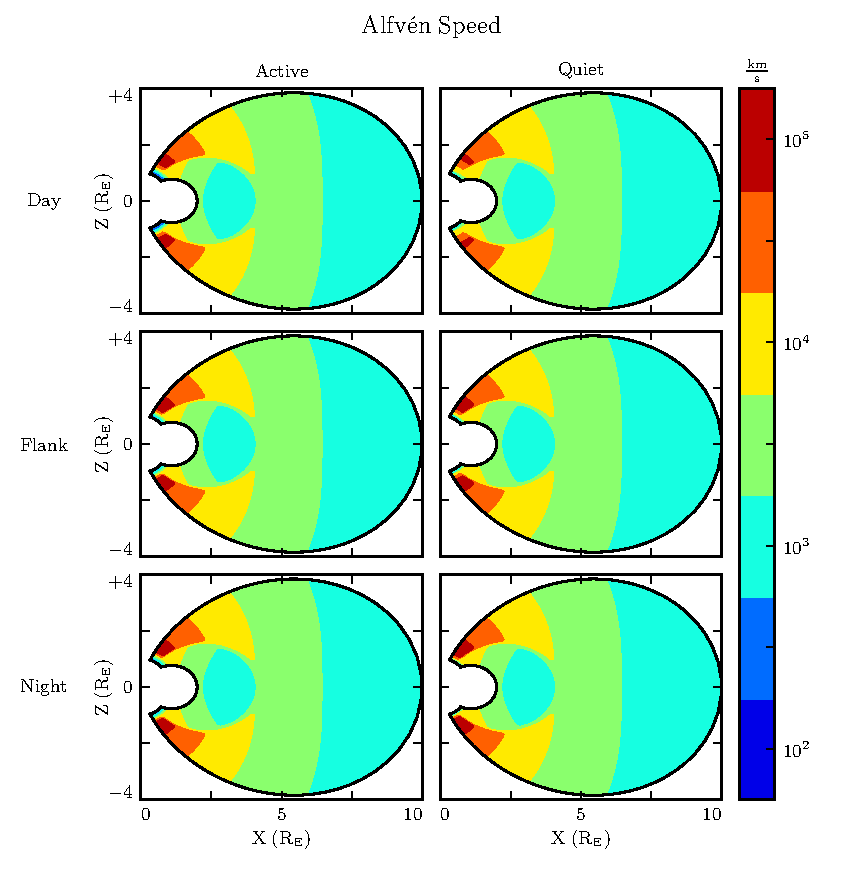
\includegraphics[width=\textwidth]{figures/va.pdf}
    \caption[\Alfven Speed Profiles]{
      \Alfven speed profiles, adapted by Lysak\cite{lysak_2013} from Appendix B of Kelley's textbook\cite{kelley_1989}. 
    }
    \label{fig_va}
\end{figure}

\todo{Above the profile, Bob scales the value that's read in as $r^5$ or something. Is there a citation for that? }

The \Alfven speed is then computed per $\va^2 \equiv \frac{1}{\mz \ep}$. 

The \Alfven speed is computed from Kelley's low-density profile, modified to take into account the local density. The density, in turn, is the sum of a plasmaspheric profile and a high-latitude auroral profile. 
\begin{align}
  \ep &= \text{(low-density tabulated value)} + \frac{ n \bar{m} }{B_0^2}
\end{align}

Where $\bar{m}$ is the ambient mean molecular mass and $B_0$ is the zeroth-order magnetic field strength, $B_0 = \SI{3.11e4}{\nano\tesla} \lr{ \frac{R_E}{r} }^3 \sqrt{ 1 + 3 \cos^2 \theta }$. Note that \SI{3.11e4}{\nano\tesla} is the value of the Earth's magnetic field at the equator on Earth's surface. 

\todo{Does Kelley list the electric constant or the \Alfven speed? }

\begin{figure}[H]
    \centering
    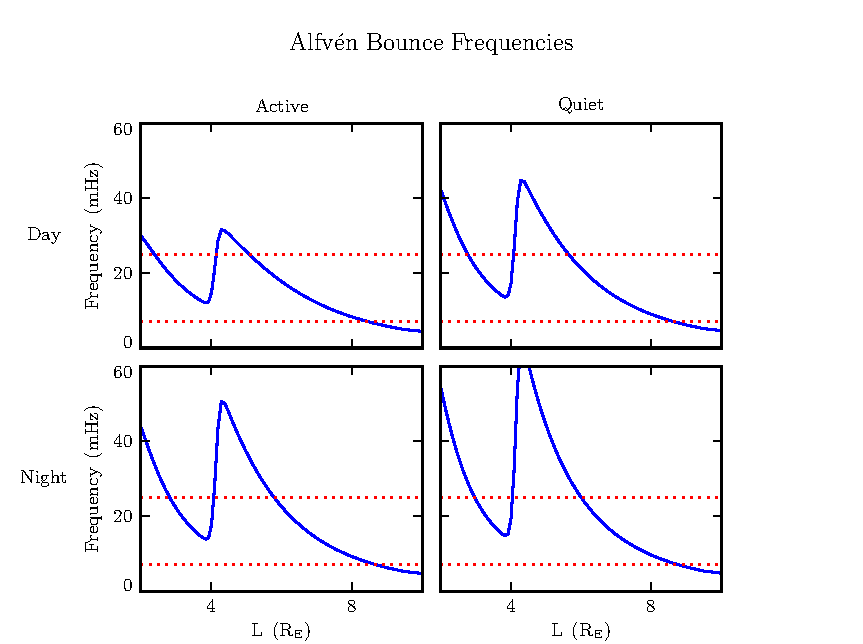
\includegraphics[width=\textwidth]{figures/fa.pdf}
    \caption[\Alfven Bounce Frequency Profiles]{
      \Alfven bounce frequency profiles, computed by integrating the the \Alfven speed back and forth over a field line. $f_A = \lrb{ \oint \frac{dz}{v_A} }^{-1}$. Dotted lines indicate the Pc4 frequency range, \SIrange{7}{25}{\mHz}. In each profile, the effect of the plasmapause is clearly visible, centered at $L=4$. Field lines just inside and just outside the plasmapause appear susceptible to resonance in the Pc4 band. 
    }
    \label{fig_fa}
\end{figure}

\todo{Talk about how the size of the plasmasphere can be adjusted, and \SI{4}{\RE} is just a typical value. }

ULF waves have been shown to correlate with pulsating aurora and with chorus\cite{jaynes_2015}. It's believed that (in the case presented) substorm injection drove Pc4-5 pulsations, which modulated chorus waves, which pitch-angle scattered electrons with energies on the order of \SI{10}{\kilo\eV}. 

\todo{Early observations of field line resonance. }

Ground signatures in the Pc4 range identified in the 1930s\cite{angenheister_1931}. Decades later, simultaneous observations at conjugate foot points of the same field line showed FLR structure\cite{sigura_1961}. And looked at their structure (?) \cite{nagata_1963}. 

\todo{Modern observations -- how do we justify using a 2.5D model? Localization in MLT. }

Pc4 pulsations are radially localized, per multiple satellite observations\cite{engebretson_1992}, and spread no more than about 8 hours MLT. They peak around $L$ of 5 to 6, with lower occurrence rate 2.5 to 9\cite{anderson_1990,liu_2009}.

\todo{Radial localization. }

The plasmapause -- representing a sharp change in \Alfven speed -- is important for ULF waves. Waves are trapped and scattered by the effective potential well, analogous to \Schrodinger's equation\cite{lee_1998,lee_1999,dai_2009}. This has been shown theoretically\cite{klimushkin_1998,leonovich_2000,klimushkin_2004,mager_2013} (most recent is \cite{mager_2013}) and observationally\cite{takahashi_2009,takahashi_2010}. 

\todo{On the generation of FLRs: }

Compressional waves come from the outer boundary, propagating across field lines\cite{lysak_1992}. 

Compressional driving doesn't preclude drift or drift-bounce resonance\cite{zong_2007,zong_2009}. 

Plasmapause refilling may cause onset of the instability that drives noncompressional Pc4s\cite{engebretson_1992,liu_2013}. 

Low \azm is compressional\cite{hughes_1994}. Drivers may include KH at the magnetopause\cite{chen_1974,southwood_1974,liu_2011}, variations in solar wind pressure (such as interplanetary shocks)\cite{zong_2007,zong_2009,hao_2014,degeling_2014,kessel_2008}, and waves in the foreshock region\cite{russell_1983,takahashi_2015}. 

AMPTE/CCE data has shown a correlation between poloidal Pc4 activity and intense ring current flux near the equator\cite{engebretson_1988}. Poloidal Pc4s may be caused by phase space gradients\cite{dai_2013}. Fundamental standing waves are possibly excited by drift resonance of ions with energy around \SI{100}{\kilo\eV}\cite{thompson_2001,dai_2013}.

``To summarize, the general buffetting of the magnetosphere by variations in the solar wind dynamic pressure, or perhaps by sporadic magnetic reconnection, provides a broad band energy source to the magnetosphere. The magnetospheric cavity as a whole rings at its own eigenfrequencies, thus transporting energy at just those frequencies to field lines deep in the magnetosphere. Those field lines whose eigenfrequencies match one of the cavity eigenfrequencies couple to the cavity mode and resonate strongly, producing the classical field line resonance signature.\cite{hughes_1994}'' 

``It is unclear whether other generation mechanisms of fundamental standing waves such as drift wave instability\cite{green_1979} can explain the localization of Pgs in local time (LT).''\cite{motoba_2015}

\todo{Observational constraints for ground-based work on FLRs: }

High-modenumber ULF pulsations are damped by the ionosphere, making it more difficult to observe them on the ground\cite{hughes_1976}. Small structures are also damped; resonances narrower than $\sim \SI{100}{km}$ aren't visible on the ground. See also Glassmeier and Stellmacher, 2000 (about small latitude), and Wright and Yeoman, 1999, Yeoman and Wright, 2001 about large \azm. 

Second harmonic poloidal waves -- as most of \cite{dai_2015}'s events are -- are unlikely to cause a Pg event on the ground\cite{takahashi_1992}. 

It's perhaps not surprising that, finding events based on ground signatures, \azm would skew low. High-\azm waves can't penetrate the ionosphere. Multi-spacecraft observation of a ULF wave with very high modenumber (70+) and no apparent ground signature\cite{takahashi_2013}. 

\todo{The ionosphere is important: }

A Hall-conducting ionosphere reflects ULF waves\cite{hughes_1974}. 

Poloidal and toroidal ULF polarizations are treated differently by the ionosphere\cite{greifinger_1968} (more recently, \cite{fujita_1988}).  

\todo{Theoretical consideration of decay vs propagation, by frequency. Lysak and Yoshikawa 2006. }

\Alfven waves with small latitudinal scale\cite{glassmeier_2000} or high \azm\cite{wright_1999,yeoman_2001} are screened by the ionosphere. Attenuation factor from \cite{hughes_1976} and \cite{glassmeier_1984} DID NOT PRINT PROPERLY. LOOK IT UP. 

Typical magnitude is order of a few nT, and a few mV/m\cite{takahashi_2013}. 

% -----------------------------------------------------------------------------
% -----------------------------------------------------------------------------
% -----------------------------------------------------------------------------
\subsection{Structure and Jargon}

\todo{Poloidal and toroidal, fundamental mode and second harmonic... make sure this vocabulary is inescapably clear! }

Drift-wave instability\cite{hasegawa_1971,green_1979,green_1985} is also a possibility for exciting fundamental poloidal waves, though it requires cold plasma, so it could only happen in the plasmasphere. 

Fundamental poloidal mode is drift resonance, not drift bounce\cite{poulter_1983}. 

Pc5 waves peak around $L$ of 7 to 9, too far out for RBSP\cite{anderson_1990,liu_2009}. Poloidal Pc4 pulsations are common inside and outside the plasmapause. Plasmapause peaks at 4.8--5 RE and 5.8--6RE\cite{dai_2015}. 

Because the inner magnetosphere is low-$\beta$ (that is, magnetic pressure dominates thermal pressure), the strength of the compressional-poloidal coupling indicates \azm\cite{hughes_1994}. 

At high \azm, the poloidal mode decouples from the compressional mode\cite{hughes_1994} and becomes guided\cite{cummings_1969}. 

Most observed guided waves are second harmonic excited by the drift-bounce resonance\cite{hughes_1978,singer_1982,takahashi_1990}. Fundamental modes, driven by drift resonance, are rarer, but have been observed\cite{dai_2013}. The energy of the resonant particle gives \azm, recall $\omega - \azm \omega_d = 0$ or something\cite{ozeke_2001}. 

A recent survey of Van Allen Probe data showed that Pc4 pulsations -- the poloidal ones, at least -- occur primarily during geomagnetically active times, near the plasmapause, over just a handful of hours of dayside MLT\cite{dai_2015}. This confirmed and refined older work\cite{engebretson_1987}. 

In the example shown of a fundamental mode poloidal Pc4, and in the example of a higher harmonic Pc4, a mishmash of toroidal activity is present. \cite{dai_2015}, figure 8 and 9 respectively. 

Compressional poloidal Pc4 pulsations are much more common during storms, but not particularly sensitive to storm phase. Noncompressional ones occur primarily during recovery\cite{dai_2015,rostoker_1979,engebretson_1992,anderson_1994}. Note that Dai\cite{dai_2015} was pretty generous about what counted as a storm... anything that hits \SI{-30}{\nano\tesla}. So \cite{motoba_2015} may not have counted the same way when they found no particular correlation with storm phase. 
\todo{Fishbone instability. McGuire 1983, Chen 1984. Similar phenomenon, but for lab plasmas. }

An ideal poloidal mode decays to the toroidal mode in the presence of curved magnetic field lines\cite{radoski_1974} or a gradient in the \Alfven speed\cite{mann_1995}. The time is proportional to the azimuthal wavenumber\cite{mann_1995}. An analytical follow-up agreed with the numerical work\cite{mann_1997}. 

\todo{Mann gives the poloidal-to-toroidal decay time to be $\tau = \frac{d \lambda}{d \omega_A'}$, where $\lambda = \frac{\azm}{2 \pi r}$ and $\omega_A'$ is the spatial derivative of the \Alfven bounce frequency, but this doesn't seem to line up. When $\tau$ is computed using our \Alfven bounce frequencies, the result is much less than \SI{1}{\second}. Double-checking is necessary. }

\cite{cummings_1969}: Standing \Alfven waves in the magnetosphere. Theoretical fundamental toroidal and poloidal modes can vary by up to \SI{30}{\percent} in frequency. 

Second harmonic: Br leads Ea by 90 degrees. Fundamental mode: Br lags Ea by 90 degrees. DEPENDS ON SIGN OF MLAT. \cite{dai_2015}

Low-\azm waves tend to be more muddled... driven by broadband sources rather than resonance\cite{dai_2015}. 

Drift resonance is the fundamental mode. Drift-bounce is higher harmonics\cite{dai_2015}. 

\todo{Do the unambiguous Pc4 events in \cite{takahashi_2011} and \cite{dai_2013} also have a mishmash of toroidal activity? }

Fundamental mode is rare. Of 390 noncompressional events, Dai identified 19 to be clearly fundamental mode and 197 to be clearly second harmonic\cite{dai_2015}. 

Fast and shear (toroidal and poloidal) modes are coupled by nonzero Hall conductivity\cite{kato_1956}. 

Shear mode incident on the ionosphere, pederson current closes FAC, Hall current then generates a fast mode wave which may be detected in space or on the ground\cite{tamao_1965}. 

Toroidal mode is usually associated with external driving\cite{chen_1974,southwood_1974}. 

Guided poloidal wave arises as \azm goes to infinity\cite{radoski_1967_poloidal}. 

Observations show that the poloidal mode is most excited in the second harmonic\cite{cummings_1969,hughes_1978,arthur_1981,singer_1982,takahashi_1984,engebretson_1988} even when there is a strong compressional component\cite{takahashi_1987,haerendel_1999,vaivads_2001,sibeck_2012}. 

Theoretical justifications for why the second harmonic would be preferrentially excited in the ring current environment\cite{southwood_1976,chen_1991,cheng_1994,chan_1994}. 

Observations of odd-mode poloidal waves... possible fundamental\cite{yang_2010,eriksson_2005}.

% -----------------------------------------------------------------------------
% -----------------------------------------------------------------------------
% -----------------------------------------------------------------------------
\subsection{Giant Pulsations}

First Pg observation\cite{birkeland_1901}. 

Pgs are most common during solar minimum, perhaps because of decreased mass loading of heavy ions\cite{denton_2011}. 

Observations in space indicate that Pgs are fundamental poloidal mode\cite{kokubun_1980,hillebrand_1982,kokubun_1989,takahashi_1992,glassmeier_1999}. 

Pgs are rare\cite{brekke_1987}. Most Pgs observed on the ground have \azm in the range 16 to 35\cite{takahashi_1992}. Motoba\cite{motoba_2015} found \azm valuse in the range 10 to 15 for a sample of Pgs. Previous studies\cite{rostoker_1979,glassmeier_1980,hillebrand_1982,poulter_1983} are in general agreement that Pg modenumbers fall into the range 16 to 35. 

Nishida\cite{nishida_1964_screening} (or maybe \cite{nishida_1964_impulses}) shows a 90 degree rotation as a long-period \Alfven wave passes through the ionosphere. That would translate a poloidal resonance in space to an east-west ground signature. 

\cite{motoba_2015} suggests that Pgs originate from the fundamental poloidal mode waves at all local times. 

``Pgs maybe a manifestation of a small subset of fundamental poloidal waves excited in the magnetopause.'' \cite{takahashi_2013}

It seems to be the convention to find a Pg event on the ground, then look at satellite data. That's certainly what was done in \cite{motoba_2015}. 

Per \cite{motoba_2015}, most Pg events happen around $L=7$, but some do happen near the plasmapause, as seen(?) by \cite{green_1985}. 

``The AL distribution shown in Figure 14c are consistent with the findings of \cite{rostoker_1979} that Pgs occur as the magnetosphere recovers from previous activities (substorms).''\cite{motoba_2015} Finds this to be reasonable because it's ``very likely'' that energetic ions injected into the inner magnetosphere from the magnetotail provide energy to Pgs. 

Analysis of GOES data from 2008 to 2013 shows about 100 Pg events. They are concentrated on the morningside. No particular correlation with storm phase\cite{motoba_2015}. 

Recall compressional poloidal Pc4s are mostly during storm time, and noncompressional are mostly specifically during late recovery\cite{dai_2015}. Only 19 fundamental poloidal mode examples were identified from the 390 noncompressional poloidal events. 

Another past study: \cite{takahashi_1984}. Satellite data is surveyed and classified by polarization, harmonic, wavenumber, etc, in order to determine the mechanisms for generating \Alfven waves. Old, but still pretty representative, according to Motoba\cite{motoba_2015}. 

% -----------------------------------------------------------------------------
% -----------------------------------------------------------------------------
% -----------------------------------------------------------------------------
\subsection{Motivations for the Present Work}

\todo{What's going on with the MLT localization of Pc4 pulsations? Is there something spooky going on with the driving? Maybe the ionosphere just kills FLRs on the nightside! }

\todo{What's so special about Pgs? How rare are they, really, compared to fundamental poloidal modes in general? How does that line up with the occurrence rate of nice, sinusoidal waveforms in second-harmonic Pc4s? That is, is there something special about Pgs, or do they just live in a ``sweet spot'' with respect to constraints on observation and resonance? }

\todo{The goal here is to clarify and unify several constraints on the viability and observability of FLRs. }

``It is not clear why noncompressional [high-\azm] Pc4 poloidal waves, which are presumably driven by instability within the magnetosphere, preferrentially occur on the dayside.\cite{dai_2015}''

``Pgs maybe a manifestation of a small subset of fundamental poloidal waves excited in the magnetopause.'' \cite{takahashi_2013}




% %%%%%%%%%%%%%%%%%%%%%%%%%%%%%%%%%%%%%%%%%%%%%%%%%%%%%%%%%%%%%%%%%%%%%%%%%%%%%
% %%%%%%%%%%%%%%%%%%%%%%%%%%%%%%%%%%%%%%%%%%%%%% Description of Numerical Model
% %%%%%%%%%%%%%%%%%%%%%%%%%%%%%%%%%%%%%%%%%%%%%%%%%%%%%%%%%%%%%%%%%%%%%%%%%%%%%

\chapter{Model}
  \label{ch_model}

\todo{The present chapter sketches the fundamental equations of waves in a cold, resistive plasma. It then illustrates the implementation of a two and a half dimensional \Alfven wave code to model those waves. Finally, takes a look at a little something extra that the code might like. }

%``Increasing the Hall conductance allows the energy to oscillate through the inductive process rather than dissipate as Joule heating, increasing the `ringtime' of field line resonances.''\cite{waters_2013}

%Ionospheric profiles are static for the duration of a simulation. Even so-called ultra low frequency waves are still much faster than convective timescales. Each profile is resolved to an altitude of about $\SI{e4}{\km}$, and include well-resolved $E$, $F_1$, and $F_2$ layers. 


  

% =============================================================================
% =============================================================================
% =============================================================================
\section{Dispersion Relation}
  \label{sec_math}

\todo{Sketch out what a dispersion relation is, why it works, why it's interesting. }

\todo{Explain that the inclusion of conductivity is novel. }

\todo{This chapter works out the sorts of waves that might be expected in the numerical model. It starts with the same equations that are used by the model -- Maxwell's equations and \ohmlaw. The resulting dispersion relation is too high-ordered for a direct solution, so several limits of interest are considered. } 

\todo{At this end of this chapter, there will be a discussion of what is specifically interesting about the findings. That doesn't really exist yet. Or... actually, should we discuss interesting things as we find them? Note that we find $\omega^2 = k^2 \va^2$ several times. }

Cold, linearlized \amplaw and \farlaw. The vector $\vec{B}$ is the perturbation to the zeroth-order magnetic field. 
\begin{align}
  \ddt \vec{B} &= -\curl{E} & \tensor{\epsilon} \cdot \ddt \vec{E} &= \oomz \curl{B} - \vec{J}
\end{align}

\ohmlaw. Electron inertial effects are included in the parallel direction. See \cref{sec_inertia}. 
\begin{align}
  \frac{\me}{n e^2} \ddt J_\parallel & = 
    \sz E_\parallel - J_\parallel &
  0 & = 
    \tensor{\sigma}_\bot \cdot \vec{E}_\bot - \vec{J}_\bot
\end{align}

Suppose that the fields and currents are resonating as $\exp \arg{i \vec{k} \cdot \vec{x} - i \omega t }$. Evaluate the derivatives. Eliminate magnetic fields and currents. 
\begin{align}
  \label{disp_setup}
\begin{alignedat}{4}
%  \label{disp_para}
  & 0 = E_\parallel && + \frac{c^2}{\omega^2} \lr{ \vec{k} \, \vec{k} \cdot \vec{E} - k^2 \vec{E} }_\parallel && + \frac{i \op^2 }{\omega \lr{\nu - i \omega} } && E_\parallel \\
%  \label{disp_perp}
  & 0 = \vec{E}_\bot && + \frac{\va^2}{\omega^2} \lr{ \vec{k} \, \vec{k} \cdot \vec{E} - k^2 \vec{E} }_\bot && + \frac{i}{\ep \omega} \tensor{\sigma}_\bot \cdot && \vec{E}_\bot
\end{alignedat}
\end{align}

The above expression makes use of the vector identity $\vec{k} \times \vec{k} \times \vec{E} = \vec{k} \, \vec{k} \cdot \vec{E} - k^2 \vec{E}$. The \Alfven speed, speed of light, plasma frequency, and parallel conductivity are defined in the usual way: 
\begin{align}
  \label{def_basics}
  \va^2 & \equiv \frac{1}{\mz \ep} &
  c^2 & \equiv \frac{1}{\mz \ez} &
  \op^2 & \equiv \frac{n e^2}{\me \ez} &
  \sz & \equiv \frac{n e^2}{\me \nu}
\end{align}

Note that this definition of the \Alfven speed takes into account the displacement current correction which is important when \va approaches $c$. 

\cref{disp_setup} is then assembled into the usual dispersion tensor form:
\begin{align}
  \label{disp}
  0 &= \lr{ \tensor{ \mathbb{I} } + \frac{1}{\omega^2} \tensor{V}^2 \cdot \vec{k} \, \vec{k} - \frac{k^2}{\omega^2} \tensor{V}^2 + \frac{i}{\omega} \tensor{\Omega} } \cdot \vec{E}
\end{align}

Where $\tensor{ \mathbb{I} }$ is the identity tensor and in \x-\y-\z coordinates, 
\begin{align}
  \tensor{V}^2 &\equiv 
    \mmm{\va^2}{0}{0}
        {0}{\va^2}{0}
        {0}{0}{c^2} &
  & \text{and} &
  \tensor{\Omega} &\equiv 
    \mmm{ \frac{\sp}{\ep} }{ \frac{-\sh}{\ep} }{0}
        { \frac{\sh}{\ep} }{ \frac{\sp}{\ep} }{0}
        {0}{0}{ \frac{\op^2}{\lr{\nu - i \omega}} } 
\end{align}

In \cref{disp}, the expression in parentheses is the dispersion tensor. Nontrivial solutions exist only when its determinant is zero. This gives rise to a seventh-order polynomial in $\omega$, so rather than a direct solution it's necessary to consider limits of specific interest. 

% -----------------------------------------------------------------------------
% -----------------------------------------------------------------------------
% -----------------------------------------------------------------------------
\subsection{Parallel or Perpendicular Propagation}
  \label{sec_par_perp}

\todo{Parallel propagation is ineresting because it's a naive representation of a field line resonance. Perpendicular propagation is interesting because the movement of energy across field lines is a topic of particular interest. In both cases, the cross terms in $\vec{k} \, \vec{k}$ vanish, decoupling the parallel and perpendicular polarizations. }

\todo{Without loss of generality, the wave vector $\vec{k}$ is presumed to lie in the \x-\z plane. The distinction between the azimuthal and crosswise directions is revisited later. }

\todo{ACTUALLY: does this even matter? If we keep $\phi$ in there in addition to $\theta$, does it cancel out? Seems like it should. }

%\subsection{Parallel Polarization}

In the parallel and perpendicular propagation limits respectively, the parallel factors of the determinants of \dispersiontensor are:
\begin{align}
  \label{parallel_math_setup}
  \begin{split}
  % Parallel propagation, parallel polarization. 
  0 &= \omega^2 + i \nu \omega - \op^2 \\
  % Perpendicular propagation, parallel polarization. 
  0 &= \omega^3 + i \nu \omega^2
  - \lr{ k^2 c^2 + \op^2 } \omega
  - i k^2 c^2 \nu
  \end{split}
\end{align}

Both expressions in \cref{parallel_math_setup} can be solved directly, though the solution to the (cubic) perpendicular propagation case is too long to be useful. After expanding with respect to a very large plasma frequency, the solutions can be written (for parallel and perpendicular propagation respectively): 
\begin{align}
  \label{parallel_math_final}
  \begin{split}
  % Parallel propagation, parallel polarization. 
  \omega^2 & = \op^2 - i \nu \op + ... \\
  % Perpendicular propagation, parallel polarization. 
  \omega^2 & = k^2 c^2 + \op^2 - i \nu \op + ...
  \end{split}
\end{align}

The first expression in \cref{parallel_math_final} -- describing the parallel-polarized component of a parallel-propagating wave -- doesn't describe a wave at all; there's no dependence on the wave vector $k$. Instead, it describes the plasma oscillation. The second expression is the O mode: a compressional wave, oscillating just above the plasma frequency, with a parallel electric field. 

The perpendicular factors of the dispersion tensor's determinant, in the cases of parallel and perpendicular propagation respectively, are: 
\begin{align}
  \label{perpendicular_math_setup}
  \begin{split}
  % Parallel propagation, perpendicular polarization. 
  0 &= \omega^4 + 2 i \frac{\sp}{\ep} \omega^3
  - \lr{ 2 k^2 \va^2 + \frac{\sp^2 + \sh^2}{\ep^2} } \omega^2
  - 2 i k^2 \va^2 \frac{\sp}{\ep} \omega
  + k^4 \va^4 \\
  % Perpendicular propagation, perpendicular polarization. 
  0 &= \omega^3 + 2 i \frac{\sp}{\ep} \omega^2
  - \lr{ 2 k^2 \va^2 + \frac{\sp^2 + \sh^2}{\ep^2} } \omega
   - i k^2 \va^2 \frac{\sp}{\ep}
  \end{split}
\end{align}

First expression of \cref{perpendicular_math_setup} can be solved directly. Noting that $\pm$ and $\opm$ are independent,
\begin{align}
  % Parallel propagation, perpendicular polarization. 
  \omega = \lr{ \frac{\pm \sh - i \sp}{2 \ep} } \opm \sqrt{ k^2 \va^2 + \lr{ \frac{\pm \sh - i \sp}{2 \ep} }^2 }
\end{align}

This wave is propagating along the field line, so the Pedersen and Hall conductivities are small for the vast majority of its trajectory. Expanding, then, gives
\begin{align}
  \label{perp_final_z}
  % Parallel propagation, perpendicular polarization. 
  \omega^2 = k^2 \va^2 \opm k \va \frac{\sh \pm i \sp}{\ep} + ...
\end{align}

The second expression of \cref{perpendicular_math_setup} can also be solved directly, though its roots are impractically long. They are expanded with respect to small conductivities (as would be seen by a perpendicular-propagating wave at high altitude) and at large conductivity (representing the perpendicular-propagating wave within the ionosphere). Respectively, 
\begin{align}
  \label{perp_final_x}
  \begin{split}
  % Perpendicular propagation, perpendicular polarization. Small conductivity. 
  \omega^2 & = k^2 \va^2 \pm i k \va \frac{\sp}{\ep} + ... \\
  % Perpendicular propagation, perpendicular polarization. Large conductivity. 
  \omega^2 & = k^2 \va^2 + \lr{ \frac{\sh \pm i \sp}{\ep} }^2 + ...
  \end{split}
\end{align}

\cref{perp_final_z,perp_final_x} describe \Alfven waves: waves traveling at the \Alfven speed (shifted by the ionospheric conductivity) with electric fields perturbations perpendicular to the zeroth-order magnetic field.  

% -----------------------------------------------------------------------------
% -----------------------------------------------------------------------------
% -----------------------------------------------------------------------------
\subsection{High Altitude Limit}
  \label{sec_high_alt}

In the limit of large radial distance, where the density is very low, it's reasonable to neglect the Pedersen conductivity, the Hall conductivity, and the collision rate. 

Without loss of generality, the wave vector $\vec{k}$ can be presumed to lie in the \x-\z plane\footnote{\todo{The azimuthal-propagation case is discussed in XXX.}}. 

Whereas in \cref{sec_par_perp} the parallel component of the determinant of the dispersion tensor could be factored out, the high altitude limit decouples the azimuthal component from those in the meridional plane. The azimuthal component gives, simply, 
\begin{align}
  \omega^2 & = k^2 \va^2
\end{align}

This solution is analogous to the results in \cref{sec_par_perp}: a wave propagating at the \Alfven speed, with electric field perturbation perpendicular to both the zeroth-order magnetic field and the wave vector. 

The meridional components of the determinant of the high-altitude limit of the dispersion tensor give: 
\begin{align}
  \label{high_meridional_setup}
  0 &= \omega^4 
  - \lr{ k_\parallel^2 \va^2 + k_\bot^2 c^2 + \op^2 } \omega^2
  + k_\parallel^2 \va^2 \op^2
\end{align}

Where $k_\parallel$ and $k_\bot$ are the parallel and crosswise components of the wave vector. The a

\cref{high_meridional_setup} is quadratic in $\omega^2$. Its solution is
\begin{align}
  \omega^2 & = \frac{1}{2} \lr{ k_\parallel^2 \va^2 + k_\bot^2 c^2 + \op^2 }
  \pm \sqrt{ \frac{1}{4} \lr{ k_\parallel^2 \va^2 + k_\bot^2 c^2 + \op^2 }^2 
    - k_\parallel^2 \va^2 \op^2 }
\end{align}

Noting that $\op$ is very large, the two roots simplify to
\begin{align}
  \label{high_meridional_final}
  \begin{split}
  \omega^2 & = k_\parallel^2 \va^2 + ... \\
  \omega^2 & = k_\parallel^2 \va^2 + k_\bot^2 c^2 + \op^2 + ...
  \end{split}
\end{align}

\todo{The first part looks like an \Alfven wave. The second is faster than the plasma frequency, so we don't really care about it. }

% -----------------------------------------------------------------------------
% -----------------------------------------------------------------------------
% -----------------------------------------------------------------------------
\subsection{Something Something Implications}
  \label{sec_implications}

\todo{High \azm limit. }

\todo{Hall conductivity? }

\todo{Waves moving at the \Alfven speed constrain time step. }



  
% =============================================================================
% =============================================================================
% =============================================================================
\section{Something Something Numerical Model}
  \label{sec_model}

\todo{This model allows arbitrary driving/propagating waveform, absorption, refraction, phase/group delay, frequency shift, polarization, faraday rotation\cite{simpson_2004,samimi_2015}. }

\todo{Sketch out this chapter. What does 2.5 dimensions mean? Why is it an appropriate approach to this problem? Why is this model in particular a good fit? What previous similar work has been done? What's novel about this mode? }

\todo{Also 2.5D: Waters 2013\cite{waters_2013}. And Waters 2008\cite{waters_2008}. }

Waters\cite{waters_2013} cites Olson\cite{olson_1978} with reference to modenumber. 

The model works in two and a half dimensions. A meridional slice of the magnetosphere is resolved. Fields are presumed to vary azimuthally according to a fixed modenumber \azm. Derivatives in $\phi$ are replaced by $i \azm$. Imaginary field values indicate a phase shift in the azimuthal direction. 

\todo{From Bob's 2013 paper\cite{lysak_2013} (which was also 2.5D): ``The shear \Alfven and compressional fast mode waves can be coupled not only by the Hall conductivity but also by inhomogeneities in the background plasma, which are unavoidable in a realistic magnetosphere [e.g., Lysak and Yoshikawa, 2006\cite{lysak_2006}; Waters et al., 2012\cite{waters_2013}]. This coupling requires a finite wave vector component in the azimuthal direction, i.e., a finite $m$ in the context of the present model. Because of the $\exp \arg{ i m \phi}$ dependence assumed in this model, the coupling from the inhomogeneity enters as an imaginary part of the coupled wave fields with respect to the initial fields, whereas the Hall conductivity appears in phase with the initial fields. Thus, although a fully three-dimensional model can give a more complete picture of wave propagation [e.g., Lysak, 2004\cite{lysak_2004}; Woodroffe and Lysak, 2012\cite{woodroffe_2012}], the present two-dimensional model serves to illustrate the nature of this coupling.''}

The use of a fixed modenumber allows a dramatic decrease in computational cost. Waves with very high azimuthal modenumber are prohibitively expensive to simulate since they can only be resolved if grid resolution is very fine in the azimuthal direction. 

\todo{Can we find a citation where someone explicitly talks about the computational cost of high-\azm simulations? Or is it just obvious Nyquist? }

This prevents the simultaneous consideration of dayside and nightside phenomena, but is fine for azimuthally-localized waves. As was shown by \cite{engebretson_1987}, and recently confirmed in detail by \cite{dai_2015}, Pc4 pulsations are generally confined to just a few hours MLT on the dayside. 

Driving with a compressional pulse from the outer boundary of a simulation is typical. This model also includes a novel driving mechanism: perturbations to the ring current. 

The code is linear. All magnetic fields are a first-order perturbation over the zeroth-order dipole field. This is a not-great assumption out towards the magnetopause. In practice, however, most activity is within $L \sim \SI{7}{\RE}$, where the dipole approximation is pretty good. 

Models with height-resolved ionospheres are a very recent development. Lysak presented his in 2013\cite{lysak_2013}. 

Ground signatures are fairly recent as well. 

\todo{Some ground signature work as far back as Greifinger and Greifinger in 1968\cite{greifinger_1968}, but there's been steady advancement. Lysak and Song, in 2006, were the first to work out ground signatures without the assumption of a single-frequency wave. }

\todo{The support software -- the driver and the plotter -- are significant too. Do they go in a section? In an appendix? }

\todo{Past FLR simulations focused on a single mode, didn't account well for the ionosphere, etc. Lee and Lysak 1989, 1990, 1991, Rankin et al 1993, 1995, 1999, Tikhonchuk and Rankin 2000, 2002. }

\todo{Past work that got ground signatures (without latitude-dependent zenith angle) Greifinger and Greifinger 1968, 1973, Hughes 1974, Sciffer and Waters 2002, Sciffer et al 2005. Better computation of ground signatures... Waters and Sciffer 2008, Sciffer and Waters 2011, Woodroffe and Lysak 2012. }

Note that the model uses megameters, seconds, megacoulombs, and grams as the fundamental units of length, time, charge, and mass respectively. As a result, electric field is measured in \si{\mV/\meter}, magnetic field is measured in \si{\nano\tesla}, and Poynting flux is measured in \si{\mW/\meter\squared}. The electric constant is expressed in \si{\milli\farad/\meter}, not in units of \ez, not that it really matters. 


% -----------------------------------------------------------------------------
% -----------------------------------------------------------------------------
% -----------------------------------------------------------------------------
\subsection{Coordinate System}
  \label{sec_coords}

\todo{Past work which could be cited for geometry examples: Radoski 1967, Lee and Lysak 1989, 1991, Rankin et al 1993, 1994, Streltsov and Lotko 1995, 1999. }

FLRs have traditionally been modeled by straightening the field lines into a rectangular configuration\cite{dungey_1954,mann_1995}, by unrolling the azimuthal coordinate into a cylindrical coordinate system\cite{radoski_1974}, or through the use of dipole coordinates\cite{radoski_1967_coords}\footnote{The dipole coordinates \radx, \rady\ and \radz are perhaps more commonly named $\mu$, $\phi$, and $\nu$ respectively; however, in the present work, $\mu$ and $\nu$ take other meanings.}:
\begin{align}
  \label{radoski_coords}
  \radx &\equiv -\frac{\sin^2 \theta}{r} &
  \rady &\equiv \phi &
  \radz &\equiv \frac{\cos \theta}{r^2}
\end{align}

Where $r$, $\theta$, and $\phi$ take on their usual spherical meanings of radial distance, colatitude, and azimuthal angle respectively. 

The dipole coordinate \radx is constant over each equipotential shell\footnote{In fact, \radx is inversely proportional to the McIlwain parameter.}, \rady is azimuthal angle, and \radz indexes each field line from south to north. The unit vectors \xhat, \yhat, and \zhat point in the crosswise\footnote{In the context of in situ measurements taken near the equatorial plane, \xhat is referred to as the radial direction; however, the present work extends the dipole grid to low altitudes, where it can be more horizontal than vertical. The term ``crosswise'' is meant to indicate that \xhat is defined by the cross product of \yhat and \zhat.} (radially outward at the equator), azimuthal (eastward), and parallel (northward at the equator) directions respectively. 






Notably, the dipole coordinates \radx, \rady, and \radz are normal to one another. While mathematically convenient, they do not readily accommodate a fixed-altitude boundary at the ionosphere, nor do they allow the dipole magnetic field to intersect the boundary at an oblique angle, as Earth's field does. As a solution, a nonorthogonal set of dipole coordinates was developed numerically by Proehl\cite{proehl_2002}, then formalized analytically by Lysak\cite{lysak_2004} in terms of their contravariant components:
\begin{align}
  \label{def_coords}
  \lysakx & = - \frac{R_I}{r} \sin^2 \theta & 
  \lysaky & = \phi &
  \lysakz & = \frac{R_I^2}{r^2} \frac{\cos \theta}{\cos \theta_0}
\end{align}

Above, $R_I$ is the position of the ionosphere relative to Earth's center; it's typically taken to be \SI{1}{\RE} + \SI{100}{\km}. 

Like the dipole coordinates \radx, \rady, and \radz, Lysak's coordinates \lysakx, \lysaky, and \lysakz correspond to $L$-shell, azimuthal angle, and position along a field line respectively. However, compared to \radz, \lysakz has been renormalized using the invariant colatitude\footnote{The invariant colatitude is the colatitude $\theta$ at which a field line intersects the ionosphere. It is related to the McIlwain parameter by $\cos\theta_0 \equiv \sqrt{1 - \frac{R_I}{L}}$. } $\theta_0$. As a result, \lysakz takes the value \num[retain-explicit-plus]{+1} at the northern ionospheric boundary and \num{-1} at the southern ionospheric boundary for all \lysakx and \lysaky. 

Because Lysak's coordinate system is not orthogonal\footnote{Curves of constant \lysakx and curves of constant \lysakz can intersect at non-right angles. }, it's necessary to consider covariant and contravariant basis vectors separately. 
\begin{align}
  \hat{e}_i & \equiv \dd{\lysaki} \vec{r} &
  \hat{e}^i & \equiv \dd{ \vec{r} } \lysaki
\end{align}

Covariant basis vectors $\hat{e}_i$ are normal to the curve defined by constant $\lysaki$, while contravariant basis vectors $\hat{e}^i$ are tangent to the coordinate curve (or, equivalently, $\hat{e}^i$ is normal to the plane defined by constant $u^j$ for all $j \ne i$). These vectors are reciprocal\footnote{The symbol $\delta^i_j$ is the Kronecker delta; the present work also makes use of the Levi-Civita symbol $\varepsilon^{ijk}$ and Einstein's convention of implied summation over repeated indeces\cite{einstein_1916}. } to one another, and can be combined to give components of the metric tensor $\tensor{g}$\cite{dhaeseleer_1991}. 
\begin{align}
  \label{def_metric}
  \hat{e}^i \cdot \hat{e}_j &= \delta^i_j &
  g_{ij} &\equiv \hat{e}_i \cdot \hat{e}_j &
  g^{ij} &\equiv \hat{e}^i \cdot \hat{e}^j 
\end{align}

The metric tensor allows rotation between covariant and contravariant representations of vectors. 
\begin{align}
  \label{metric}
  A_i &= g_{ij} A^j &
  & \text{and} &
  A^i &= g^{ij} A_j &
  & \text{where} &
  A_i &\equiv \vec{A} \cdot \hat{e}_i &
  & \text{and} &
  A^i &\equiv \vec{A} \cdot \hat{e}^i
\end{align}

In addition, the determinant of the metric tensor\footnote{Note $g \equiv \det \tensor{g}$. } is used to define cross products and curls\footnote{The quantity \jac is called the Jacobian determinant. It's sometimes denoted using the letter $J$, which the present work reserves for current.}. 
\begin{align}
  \label{jacobian}
  \lr{ \cross{A}{B} }^i &= \frac{ \varepsilon^{ijk} }{\jac} A_j B_k &
  & \text{and} &
  \lr{ \curl{A} }^i &= \frac{ \varepsilon^{ijk} }{\jac} \dd{\lysakj} A_k &
  & \text{where} &
  \jac &= \sqrt{g}
\end{align}

Explicit forms of the basis vectors and metric tensor can be found in the appendix of \cite{lysak_2004}. At present, it's sufficient to note the mapping between Lysak's basis vectors and the usual dipole unit vectors. 
\begin{align}
  \label{def_xyz_directions}
  \xhat &= \frac{1}{ \sqrt{ g^{11} } } \hat{e}^1 &
  \yhat &= \frac{1}{ \sqrt{ g^{22} } } \hat{e}^2 &
  \zhat &= \frac{1}{ \sqrt{ g_{33} } } \hat{e}_3
\end{align}

The basis vectors can also be mapped to the spherical unit vectors, though \cref{def_rqf_directions} is valid only at the ionospheric boundary. 
\begin{align}
  \label{def_rqf_directions}
  \qhat &= \frac{1}{ \sqrt{ g_{11} } } \hat{e}_1 &
  \fhat &= \frac{1}{ \sqrt{ g_{22} } } \hat{e}_2 &
  \rhat &= \frac{1}{ \sqrt{ g^{33} } } \hat{e}^3
\end{align}


The coordinates converge at the equatorial ionosphere, so an inner boundary is necessary to maintain finite grid spacing. It's typically placed at $L=2$. The outer boundary is at $L=10$. The dipole approximation of Earth's magnetic field is tenuous at the outer boundary (particularly on the dayside); however, in practice, wave activity is localized inside $L\sim7$. The grid is spaced uniformly in \lysakx, which gives finer resolution close to Earth and coarser resolution at large distances. 

Spacing in \lysakz is set by placing grid points along the outermost field line. The points are closest together at the ionosphere, and grow towards the equator. The spacing increases in a geometric fashion, typically by \SI{3}{\percent}. 

Most simulations take the grid to be 150 points in \lysakx by 350 points in \lysakz. The result is a resolution on the order of \SI{10}{\km} at the ionosphere, which increases to the order of \SI{e3}{\km} at the midpoint of the outermost field line. 

There are no grid points in \lysaky, of course, because of the two and a half dimensional nature of the model. Fields are assumed to vary as $\exp \arg{i \azm \lysaky}$, so derivatives with respect to \lysaky are equivalent to a factor of $i \azm$. In effect, this means that the real component of each field is azimuthally in phase with the (purely real) driving, while imaginary values represent behavior that is azimuthally offset. 

\begin{figure}[H]
    \centering
    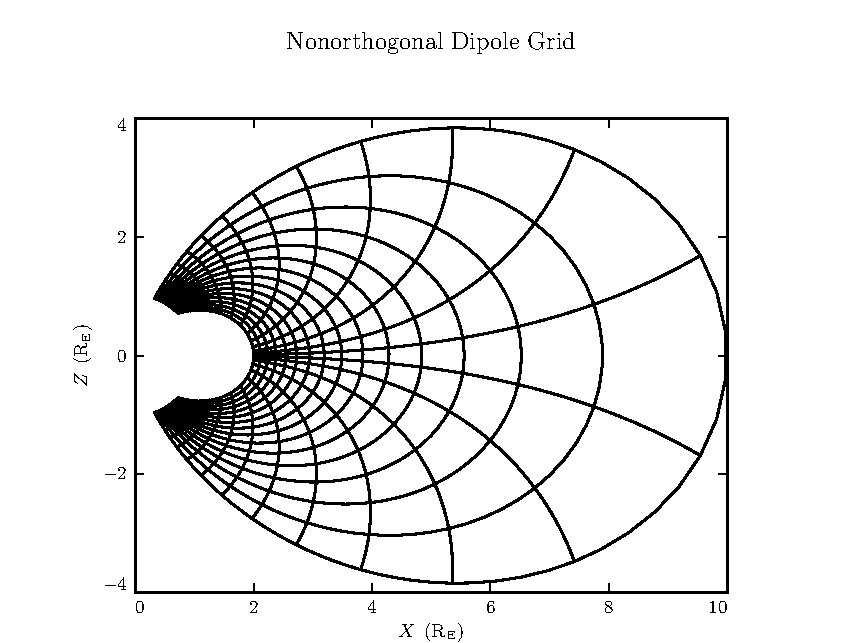
\includegraphics[width=\textwidth]{figures/grid.pdf}
    \caption[Nonorthogonal Dipole Grid]{
      The model's nonorthorthogonal dipole grid. Every fifth point is shown in each direction. The high concentration of grid points near Earth's equator is a consequence of the coordinate system, which converges at the equatorial ionosphere. 
    }
    \label{fig_grid}
\end{figure}

The simulation's time step is set based on the grid spacing. As is the convention, \dt is set to match the smallest \Alfven zone crossing time, scaled down by a Courant factor (typically 0.1). It bears noting that the smallest crossing time need not correspond to the smallest zone; recall from \cref{fig_va} that the \Alfven speed is very high in the Ionospheric \Alfven Resonator. A typical time step is on the order of \SI{e-5}{\second}. 

\todo{Do we need a citation for how time steps are set based on crossing times? }

% -----------------------------------------------------------------------------
% -----------------------------------------------------------------------------
% -----------------------------------------------------------------------------
\subsection{Maxwell's Equations}
  \label{sec_eqns}

\todo{Introduce \farlaw and \amplaw, respectively, after using Kirchhoff's formulation of \ohmlaw ($\vec{J} = \tensor{\sigma} \cdot \vec{E}$) to eliminate explicit curl dependence... which is revisited in \cref{sec_inertia}. }
\begin{align}
  \label{def_eqns}
  \ddt \vec{B} &= - \curl{E} &
  \tensor{\epsilon} \cdot \ddt \vec{E} &= \frac{1}{\mu_0} \curl{B} - \tensor{\sigma} \cdot \vec{E}
\end{align}

\todo{Explain that we'll start in \x-\y-\z coordinates -- crosswise, azimuthal, and parallel -- then map to the nonorthogonal basis at the very end. Otherwise it's necessary to carry around geometric factors. }

\todo{Leapfrog grid (for which Waters\cite{waters_2013} cites Taflove and Hagness, an electrodynamics textbook). Talk about the grid parity as well as the offset in time. }

%Field values are offset to ensure that most differences are centered. For example, $\ddt B_2$ depends on $\dd{\lysakx} E_3$ and $\dd{\lysakz} E_1$. If $B_2$ is defined at even $i$, $E_3$ is defined at odd $i$, so that $B_2$ is defined on the same grid points as $\frac{ E_3 \lrb{i+1} - E_3 \lrb{i-1} }{ \lysakx \lrb{i+1} - \lysakx \lrb{i-1} }$. 

%\todo{Make sure the example uses the currect parities. }

%\todo{Find a citation for the wigglies that occur if field values are defined on all grid points, due to the weak coupling. This problem is apparently well-known. }

%Values are sometimes needed off-parity. $E_1$ and $E_2$ are not defined at the same grid locations, but they are coupled directly by the Hall conductivity. And $B_1$ and $B_3$ are coupled by the non-orthogonality of the grid. When off-parity values are needed, they are interpolated from their neighbors. 

%Differentiation and interpolation are good to second order on the nonuniform grid. Like the coefficients for Maxwell's equations, differentiation and interpolation weights are computed during setup to save time during iteration. 

%\begin{align}
%  \label{def_assign}
%  \begin{split}
%  \int_0^{\dt} \! dt \, \ddt \vec{B} &= - \displaystyle\int_0^{\dt} \! dt \, \curl{E} \\ 
%  \left. \vec{B} \right|_{\dt} - \left. \vec{B} \right|_0 &= \left. - \dt \, \curl{E} \right|_{ \frac{\dt}{2} } \\
%  \vec{B} &\assign \vec{B} - \dt \, \curl{E}
%  \end{split}
%\end{align}

\todo{Precomputation of coefficients. }

\todo{Curl shorthand, \vec{C} and \vec{F}. Recalling \cref{jacobian}, }
\begin{align}
  \label{def_curls}
  C^i & = \frac{ \varepsilon^{ijk} }{\jac} \dd{\lysakj} E_k &
  F^i & = \frac{ \varepsilon^{ijk} }{\jac} \dd{\lysakj} B_k
\end{align}

\todo{OpenMP. }

\todo{Keeping only covariant field components and contravariant curl components, since we only use contravariant coordinates. }




Taking the shorthand introduced in \cref{def_curls}, \farlaw can simply be written: 
\begin{align}
  \label{farlaw_ijk}
  \ddt B^i &= - C^i
\end{align}

Writing each component out explicitly, and using the metric tensor (per \cref{metric}) to eliminate contravariant magnetic field components, \cref{farlaw_ijk} becomes:
\begin{align}
  \label{farlaw_final}
  \begin{split}
  B_1 &\assign B_1 - g_{11} \, \dt \, C^1 - g_{13} \, \dt \, C^3 \\
  B_2 &\assign B_2 - g_{22} \, \dt \, C^2 \\
  B_3 &\assign B_3 - g_{31} \, \dt \, C^1 - g_{33} \, \dt \, C^3
  \end{split}
\end{align}

Note that the \assign operator is used in \cref{farlaw_final} to indicate assignment, rather than equality. Terms on the left are new, while those on the right are old. 






\amplaw, as formulated in \cref{def_eqns}, presents a nontrivial differential equation. Not only are the electric field values coupled to their own derivatives, but the crosswise and azimuthal components of the equation are coupled by the Hall terms in the conductivity tensor. 

\todo{``The derivative of \vec{J} depends on the future value of \vec{j}.'' }

Fortunately, the permittivity tensor can be easily inverted, allowing a solution by integrating factor. Recalling the shorthand introduced in \cref{def_curls},
\begin{align}
  \label{int_fac_0}
  \tensor{\epsilon} \cdot \ddt \vec{E} &= \frac{1}{\mu_0} \vec{F} - \tensor{\sigma} \cdot \vec{E} &
  & \text{becomes} &
  \lr{ \tensor{\Omega} + \tensor{ \mathbb{I} } \ddt } \cdot \vec{E} &= \tensor{V}^2 \cdot \vec{F}
\end{align}

Where $\tensor{ \mathbb{I} }$ is the identity tensor and in \x-\y-\z coordinates\footnote{Note the parallel component of the present definition of $\tensor{\Omega}$ differs slightly from that used in \cref{sec_math}.}, 
\begin{align}
  \tensor{V}^2 &\equiv \frac{1}{\mz} \tensor{\epsilon}^{-1} = 
    \mmm{\va^2}{0}{0}
        {0}{\va^2}{0}
        {0}{0}{c^2}
  && \text{and} &
  \tensor{\Omega} &\equiv \tensor{\epsilon}^{-1} \cdot \tensor{\sigma} = 
    \mmm{ \frac{\sp}{\ep} }{ \frac{-\sh}{\ep} }{0}
        { \frac{\sh}{\ep} }{ \frac{\sp}{\ep} }{0}
        {0}{0}{ \frac{\sz}{\ez} } 
\end{align}

Multiplying through by $\exp \arg{ \tensor{\Omega} \, t }$ and applying the product rule, \cref{int_fac_0} becomes\footnote{Tensor exponentiation is analogous to scalar exponentiation\cite{hall_2015}: $\exp \arg{ \tensor{T} } \equiv \displaystyle\sum_n \frac{1}{ n! } \tensor{T}^n$.}
\begin{align}
  \label{int_fac_1}
  \ddt \Big( \exp \arg{\tensor{\Omega} \, t} \cdot \vec{E} \, \Big) &= \exp \arg{\tensor{\Omega} \, t} \cdot \vec{V}^2 \cdot \vec{F}
\end{align}

\cref{int_fac_1} can then be integrated over a small time step \dt and expressed in terms of the assignment operator introduced in \cref{farlaw_ijk}. 
\begin{align}
  \label{int_fac_2}
  \vec{E} &\assign \exp \arg{ -\tensor{\Omega} \, \dt } \cdot \vec{E} + \dt \, \exp \arg{ -\tensor{\Omega} \, \tfrac{\dt}{2} } \cdot \tensor{V}^2 \cdot \vec{F}
\end{align}

The tensor exponential can be evaluated by splitting $\tensor{\Omega}$ into the sum of its diagonal and Hall components\footnote{As long as the tensors $\tensor{T}$ and $\tensor{T}'$ commute -- which is guaranteed if either is diagonal -- $\exp \arg{ \tensor{T} + \tensor{T}' } = \exp \arg{ \tensor{T} } \exp \arg{ \tensor{T}' }$. }. The Hall exponential condenses into sines and cosines, giving a rotation around the magnetic field line. 
\begin{align}
  \label{amp_final}
  \vec{E} &\assign \exp \arg{ -\tensor{\Omega}_D \; \dt } \cdot \tensor{R}_z \arg{ \tfrac{-\sh \dt}{\ep} } \cdot \vec{E}
   + \dt \, \tensor{V}^2 \cdot \exp \arg{ -\tensor{\Omega}_D \; \tfrac{\dt}{2} } \cdot \tensor{R}_z \arg{ \tfrac{-\sh \dt}{2 \ep} } \cdot \vec{F}
\end{align}

Where 
\begin{align}
  \tensor{R}_z \arg{\theta} &= 
  \mmm{\cos\theta}{-\sin\theta}{0}
      {\sin\theta}{\cos\theta}{0}
      {0}{0}{1} &
  & \text{and} &
  \tensor{\Omega}_D &\equiv
    \mmm{ \frac{\sp}{\ep} }{0}{0}
        {0}{ \frac{\sp}{\ep} }{0}
        {0}{0}{ \frac{\sz}{\ez} }
\end{align}

The parallel component of term of \cref{amp_final} is simply
\begin{align}
  E_\parallel \assign E_\parallel \exp \arg{ \tfrac{- \sz \dt}{\ez} } + c^2 \dt F_\parallel \exp \arg{ \tfrac{- \sz \dt}{2 \ez} }
\end{align}

Or, in covariant terms, 
\begin{align}
  \label{e3_final}
  E_3 \assign E_3 \exp \arg{ \tfrac{- \sz \dt}{\ez} } + c^2 \dt \lr{ g_{31} F^1 + g_{33} F^3 } \exp \arg{ \tfrac{- \sz \dt}{2 \ez} }
\end{align}

Using the conductivity profiles introduced in \cref{sec_ionos}, the minimum value of $\frac{\sz \dt}{\ez}$ is on the order of \num{e3}, making $\exp \arg{ \frac{- \sz \dt}{\ez} }$ far too small to be stored in a double precision variable\footnote{Not coincidentally, $\frac{\sz}{\ez}$ can also be written $\frac{\op^2}{\nu}$. At the ionosphere, the collision frequency $\nu$ is fast compared to the frequency of a ULF wave... but it's still slow compared to the plasma frequency.}. That is, this model takes $E_3$ (and, proportionally, $E_\parallel$) to be uniformly zero. This issue is revisited in \cref{sec_inertia}. 

The perpendicular components of \cref{amp_final}, mapped from the dipole basis to the covariant basis using \cref{def_xyz_directions} and \cref{metric}, give the expressions: 
\begin{alignat}{6}
  \label{e1_final}
  & E_1 + \frac{ g^{13} }{ g^{11} } && E_3 \assign &&   && E_1 && \cos \arg{ \tfrac{- \sh \dt}{\ep} } \exp \arg{ \tfrac{- \sp \dt}{\ep} } &&  \notag \\
  &                                 &&             && + && E_2 && \sin \arg{ \tfrac{- \sh \dt}{\ep} } \exp \arg{ \tfrac{- \sp \dt}{\ep} } &&  \sqrt{ \frac{ g^{22} }{ g^{11} } } \notag \\
  &                                 &&             && + && E_3 && \cos \arg{ \tfrac{- \sh \dt}{\ep} } \exp \arg{ \tfrac{- \sp \dt}{\ep} } &&  \frac{ g^{13} }{ g^{11} } \\
  &                                 &&             && + && F^1 && \cos \arg{ \tfrac{- \sh \dt}{2\ep} } \exp \arg{ \tfrac{- \sp \dt}{2\ep} } &&  \frac{\va^2 \dt}{ g^{11} } \notag \\
  &                                 &&             && + && F^2 && \sin \arg{ \tfrac{- \sh \dt}{2\ep} } \exp \arg{ \tfrac{- \sp \dt}{2\ep} } &&  \frac{\va^2 \dt}{ \sqrt{ g^{11} g^{22} } } \notag \\
  \intertext{and}
  \label{e2_final}
  & && E_2 \assign && - && E_1 && \sin \arg{ \tfrac{- \sh \dt}{\ep} } \exp \arg{ \tfrac{- \sp \dt}{\ep} } &&  \sqrt{ \frac{ g^{11} }{ g^{22} } } \notag \\
  & &&             && + && E_2 && \cos \arg{ \tfrac{- \sh \dt}{\ep} } \exp \arg{ \tfrac{- \sp \dt}{\ep} } &&  \notag \\
  & &&             && - && E_3 && \sin \arg{ \tfrac{- \sh \dt}{\ep} } \exp \arg{ \tfrac{- \sp \dt}{\ep} } &&  \frac{ g^{13} }{ \sqrt{ g^{11} g^{22} } } \\
  & &&             && - && F^1 && \sin \arg{ \tfrac{- \sh \dt}{2\ep} } \exp \arg{ \tfrac{- \sp \dt}{2\ep} } &&  \frac{\va^2 \dt}{ \sqrt{ g^{11} g^{22} } } \notag \\
  & &&             && + && F^2 && \cos \arg{ \tfrac{- \sh \dt}{2\ep} } \exp \arg{ \tfrac{- \sp \dt}{2\ep} } &&  \frac{\va^2 \dt}{ g^{22} } \notag
\end{alignat}

Note that the $E_3$ terms can be ignored at present. They are referenced in \cref{sec_inertia}. 



% -----------------------------------------------------------------------------
% -----------------------------------------------------------------------------
% -----------------------------------------------------------------------------
\subsection{Driving}
  \label{sec_driving}


\todo{If no energy is added, the simulation is pretty boring. Everything just stays zero. }




\todo{It's traditional to drive from the outer boundary. Cite some examples. It's an analog for solar wind conditions. The analogy is clear at low modenumbers (large azimuthal wavelengths), but is plausible at high modenumber (small azimuthal wavelengths) as well, due to KH waves on the magnetopause, for example. }

\todo{As discussed in \cref{sec_flrs} and again in XXX, \Alfven waves become guided as the azimuthal modenumber becomes large. Energy delivered at the outer boundary, as a result, is unable to propagate across field lines to stimulate resonances in the inner magnetosphere.}

\todo{Compressional driving is applied by setting the value of $B_3$ at the boundary. A typical scale is \SI{10}{\nano\tesla}. }

\todo{\cref{fig_bdrive} demonstrates this issue. Note that the large values on the bottom row should be taken with a grain of salt; it's not clear that the simulation is reliable when waves are continuously forced against the boundary. }

\begin{figure}[H]
    \centering
    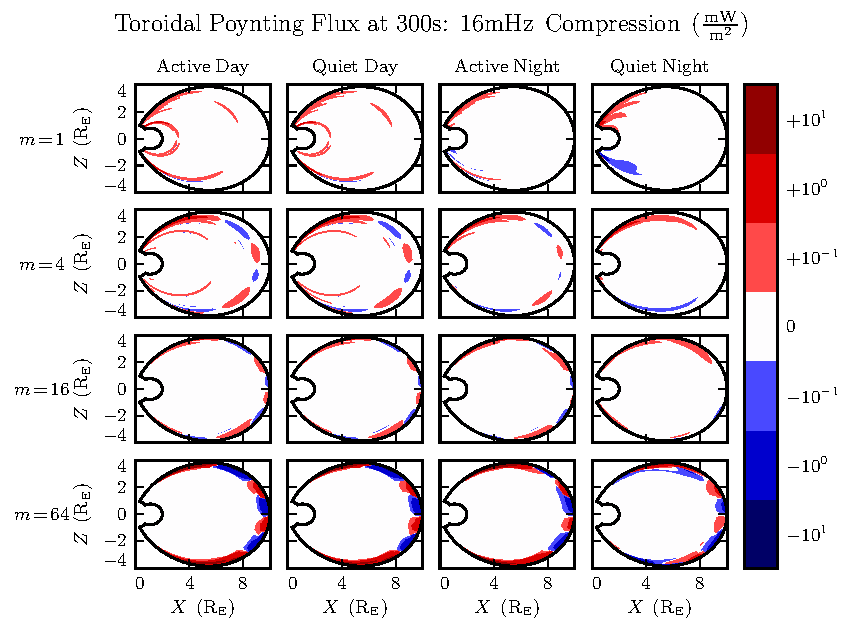
\includegraphics[width=\textwidth]{figures/bdrive.pdf}
    \caption[Decreasing Penetration with Increasing Modenumber]{
      When the azimuthal modneumber is small, energy delivered through compression at the outer boundary propagates across field lines to stimulate resonances in the inner magnetosphere. However, as modenumber increases, \Alfven waves become increasingly guided. As a result, the inner magnetosphere is unaffected by perturbations at the outer boundary. 
    }
    \label{fig_bdrive}
\end{figure}

\todo{The present work, as a result, focuses mostly on simulations driven from within the magnetosphere. }






\todo{Pc4 pulsations with high azimuthal modenumber have been shown to originate within the magnetosphere, such as through drift-resonant interactions with energetic radiation belt and ring current particles. Substorm injection can cause localized ring current behavior. }

\todo{During and after geomagnetically active times, the ring current is a dynamic region. It's easy to imagine localized perturbations, though difficult to estimate their scale. The following is a kludgey estimate -- better than no estimate at all! }

\todo{The Sym-H storm index\cite{nasa_cdaweb} measures magnetic perturbations on Earth's surface due to ring current activity. It's measured once per minute\footnote{Dst, the more commonly used storm index, is measured hourly. }, so Fourier amplitudes in the Pc4 range cannot be measured directly. However, they can be inferred by fitting the pink noise distribution. \cref{fig_symh} shows a Fourier series of the June 2013 storm and its recovery, along with its Fourier series coefficients. The red line shows a fit along the maximum of the Fourier coefficients. }

\todo{Note that Sym-H is global and we're looking at localized perturbations! This is a conservative estimate, because it's averaged over the entire globe. Information on modenumbers comes from observations by Dai\cite{dai_2015} and Takahashi\cite{takahashi_2013}, both of whom have seen fundamental-mode Pc4 pulsations with modenumbers of $\sim\num{70}$. }

\begin{figure}[H]
    \centering
    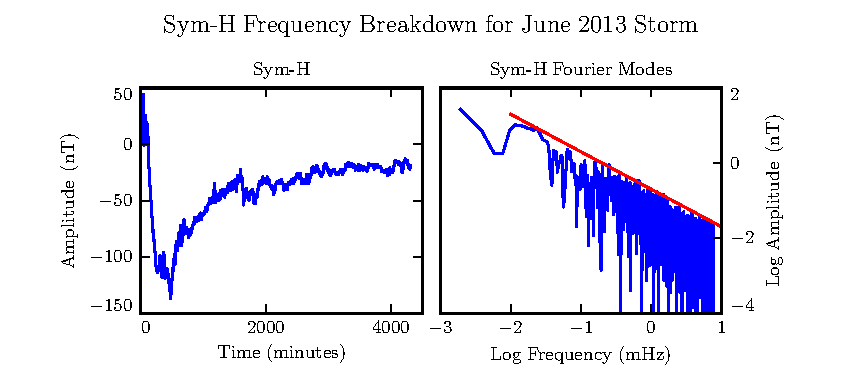
\includegraphics[width=\textwidth]{figures/symh.pdf}
    \caption[Sym-H Fourier Components for June 2013 Storm ]{
      The Sym-H storm index\cite{nasa_cdaweb} measures magnetic perturbations on Earth's surface due to ring current activity. The amplitude of oscillations in the Pc4 range is estimated by fitting the Fourier amplitudes of the June 2013 storm. 
    }
    \label{fig_symh}
\end{figure}

\todo{$\tilde{B} \arg{f} \sim \SI{e-2}{\nano\tesla} \lr{ \frac{ \SI{20}{\mHz} }{f} }$. }

\todo{An oscillation with a period of about a minute could have an amplitude on the order of \SI{e-2}{\nano\tesla}. }

\todo{Driving is typically delivered at $L=5$, with a Gaussian spread of \SI{0.5}{\RE} radially and \SI{5}{\degree} in latitude. Estimating the geometric factors from the size of the ring current, and from the fact that Sym-H is measured at Earth's surface rather than at the center of the ring, this gives current density on the order of \SI{e-4}{\uA/\meter\squared}. }

\todo{The driving current is applied by splitting the current in \amplaw into an Ohmic term and a driving term: 
\begin{align}
  \tensor{\epsilon} \cdot \ddt \vec{E} &= \frac{1}{\mu_0} \curl{B} - \tensor{\sigma} \cdot \vec{E} - \vec{J}_{drive}
\end{align}
\cref{def_curls} is then ammended so that $\vec{F} \equiv \curl{B} - \vec{J}_{drive}$. As a result, no changes are necessary to \cref{e1_final,e2_final,e3_final}. 
}

\todo{Effective peak driving electric field is... }

% -----------------------------------------------------------------------------
% -----------------------------------------------------------------------------
% -----------------------------------------------------------------------------
\subsection{Boundary Conditions}
  \label{sec_bcs}

\todo{The grid can't go on forever. There have to be special cases at the edges. }






\todo{Recall that parity was already discussed. }

Dirichlet and Neumann boundary conditions are applied to the electric field components and magnetic field components respectively. That is, electric fields are forced to go to zero at the inner and outer boundaries, and magnetic fields are forced to have a zero derivative normal to the inner and outer boundaries. 

These boundary conditions can in principle cause nonphysical reflections at the boundary\footnote{See, for example, the bottom row of \cref{fig_bdrive}. }. However, in practice, wave activity is concentrated well within the simulation domain. Simulation results are robust under an exchange of Dirichlet and Neumann boundary conditions (though a self-inconsistent set of boundary condidtions, such as applying Neumann boundary conditions to $B_1$ but Dirichlet boundary conditions to $B_3$, quickly causes instability). 





Between the top of the neutral atmosphere and the bottom of the ionosphere, the model includes a thin, horizontal current sheet representing the ionosphere's $E$ layer\cite{lysak_2004}. By integrating \amplaw over the layer, it can be shown\cite{fujita_1988} that the horizontal electric field values at the edge of the grid are determined by the jump in the horizontal magnetic fields:
\begin{align}
  \label{jump_condition}
  \tensor{\Sigma} \cdot \vec{E} &= \frac{1}{\mz} \, \displaystyle\lim_{\dr \rightarrow 0} \, \bigg[ \, \hat{r} \! \times \! \vec{B} \, \bigg|^{R_I + \dr}_{R_I - \dr}
\end{align}

Like the height-resolved conductivities in \cref{sec_eqns}, the tensor $\tensor{\Sigma}$ is based on Kelley's\cite{kelley_1989} conductivity profiles. Parallel, Pedersen, and Hall conductivities are integrated from Earth's surface to the ionospheric boundary, then arranged (in $\theta$-$\phi$ coordinates) as\cite{lysak_2004}:
\begin{align}
  \label{def_sigma}
  \tensor{\Sigma} &\equiv \mm{ \frac{\Sigma_0 \Sigma_P}{ \Sigma_0 \cos^2 \alpha + \Sigma_P \sin^2 \alpha } }{ \frac{-\Sigma_0 \Sigma_H}{ \Sigma_0 \cos^2 \alpha + \Sigma_P \sin^2 \alpha } }
                             { \frac{\Sigma_0 \Sigma_H}{ \Sigma_0 \cos^2 \alpha + \Sigma_P \sin^2 \alpha } }{ \Sigma_P + \frac{\Sigma_H^2 \sin^2 \alpha}{ \Sigma_0 \cos^2 \alpha + \Sigma_P \sin^2 \alpha } } \end{align}

Where $\alpha$ is the angle between the magnetic field and the vertical direction, given by $\cos \alpha \equiv \frac{ -2 \cos \theta }{ \sqrt{1 + 3 \cos^2\theta} }$. 

An expression for the horizontal electric fields at the boundary can be obtained by inverting \cref{jump_condition}. After mapping to covariant coordinates per \cref{def_rqf_directions}, and taking $\Sigma \equiv \det \tensor{\Sigma}$,
\begin{align}
  \label{eatm_final}
  \begin{alignedat}{6}
  & E_1 \assign \frac{1}{\mz \Sigma} \, \displaystyle\lim_{\dr \rightarrow 0} \, \bigg[ \, &- & \Sigma_{\theta\phi} && B_1   && - \sqrt{ \frac{ g_{11} }{ g_{22} } }&&\Sigma_{\phi\phi} && B_2 \, \bigg|^{R_I + \dr}_{R_I - \dr} \\
  & E_2 \assign \frac{1}{\mz \Sigma} \, \displaystyle\lim_{\dr \rightarrow 0} \, \bigg[ \, &\sqrt{ \frac{ g_{22} }{ g_{11} } } & \Sigma_{\theta\theta} && B_1 && +  &&\Sigma_{\phi\theta} && B_2 \, \bigg|^{R_I + \dr}_{R_I - \dr}
  \end{alignedat}
\end{align}

The atmospheric magnetic field is computed as a linear combination of harmonics. The neutral atmosphere is considered to be a perfect insulator, giving $\curl{B}=0$. Combined with $\div{B}=0$ (per Maxwell's equations), this allows the computation of a magnetic scalar potential $\Psi$ such that $\vec{B}=\grad{\Psi}$ and $\Psi$ satisfies Laplace's equation, $\nabla^2 \Psi = 0$. 

Laplace's equation can be solved analytically; however, a numerical solution is preferrable to ensure orthonormality on a discrete and incomplete\footnote{As discussed in \cref{sec_coords}, the grid is constrained to finite $L$, which excludes the equator as well as the poles. } grid. After separating out the radial and azimuthal dependence in the usual way, the latitudinal component of Laplace's equation can be written in terms of $s \equiv - \sin^2 \theta$: 
\begin{align}
  \label{laplace}
  \lr{ 4 s^2 + 4s } \frac{d^2}{ds^2} Y_\ell + \lr{ 4 + 6 s } \frac{d}{ds} Y_\ell - \frac{\azm^2}{s} Y_\ell &= \ell \, \lr{ \ell + 1 } Y_\ell
\end{align}

Using centered differences to linearize the derivatives, \cref{laplace} becomes a system of coupled linear equations, one per field line. It can be solved numerically for eigenvalues $\ell \, \lr{\ell + 1}$ and eigenvectors\footnote{The eigenvectors are not vectors in the same sense as \vec{B} and \vec{E}, of course; rather, they are scalar functions of $\theta$ defined on a discrete grid. } $Y_\ell$\footnote{Solving Laplace's equation analytically results in spherical harmonics indexed by both $\ell$ and \azm, the separation constants for $\theta$ and $\phi$ respectively. In two and a half dimensions, $\phi$ is not explicitly resolved, so \azm is set manually.}. In terms of the harmonics $Y_\ell$, $\Psi$ between the Earth's surface and the top of the atmosphere can be written
\begin{align}
  \label{psi_expansion}
  \Psi \arg{r, \theta} &= \displaystyle\sum_\ell \lr{ a_\ell \, r^\ell + b_\ell \, r^{-\ell - 1} } Y_\ell \arg{\theta}
\end{align}

As a boundary condition for $\Psi$, Earth is assumed to be a perfect conductor. This forces the magnetic field at Earth's surface to be horizontal; that is, $B_r = \dd{r} \Psi = 0$. Noting that solutions to Laplace's equation are orthonormal, each element of the sum in \cref{psi_expansion} must be independently zero at $R_E$. This allows the coefficients $a_\ell$ and $b_\ell$ to be expressed in terms of one another. 
\begin{align}
  \label{beta_solution}
  b_\ell &= \frac{\ell}{\ell + 1} R_E^{2 \ell + 1} a_\ell
\end{align}

The current sheet at the top of the atmosphere has been assumed to be horizontal, so the radial component of the magnetic field must be the same just above and just below it. Taking the radial derivative of \cref{psi_expansion} at the top of the atmosphere, and eliminating $b_\ell$ with \cref{beta_solution}, gives
\begin{align}
  B_r &= \displaystyle\sum_\ell \ell \, a_\ell \, R_I^{\ell-1} \, \lr{ 1 - \lambda_I^{2 \ell + 1} } Y_\ell &
  & \text{where} &
  \lambda_I &\equiv \frac{R_E}{R_I} \sim \num{0.975}
\end{align}

The summation can be collapsed by ``integrating'' over a harmonic\footnote{Because the functions are defined on a discrete grid, their inner product is not an integral, but a sum: $B_r \cdot Y_\ell^{-1} \equiv \displaystyle\sum_i B_r [i] \; Y_\ell^{-1} \! [i] $. }. Inverse harmonics can be obtained by inverting the eigenvector matrix. Then $Y_\ell \cdot Y_{\ell'}^{-1} = \delta_{\ell \ell'}$ by construction. 
\begin{align}
  \label{alpha_solution}
  a_\ell &= \frac{ 1 }{\ell \, R_I^{\ell-1} } \frac{ B_r \cdot Y_\ell^{-1} }{ 1 - \lambda_I^{2 \ell + 1} }
\end{align}

Combining \cref{psi_expansion,beta_solution,alpha_solution} allows the expression of $\Psi$ at the top and bottom of the atmosphere as a linear combination of radial magnetic field components at the bottom of the ionosphere. 
\begin{align}
  \label{psi_final}
  \begin{split}
  \Psi_E &= \displaystyle\sum_\ell Y_\ell \; \frac{R_I}{\ell} \frac{ \frac{2 \ell - 1}{\ell - 1} \lambda^\ell }{ 1 - \lambda_I^{2 \ell + 1} } B_r \cdot Y_\ell^{-1} \\
  \Psi_I &= \displaystyle\sum_\ell Y_\ell \; \frac{R_I}{\ell} \frac{ 1 + \frac{\ell}{\ell - 1} \lambda_I^{2 \ell + 1} }{ 1 - \lambda_I^{2 \ell + 1} } B_r \cdot Y_\ell^{-1}
  \end{split}
\end{align}

Horizontal magnetic fields are obtained by taking derivatives of $\Psi$. 
\begin{align}
  B_1 &= \dd{\lysakx} \Psi &
  B_2 &= \dd{\lysaky} \Psi
\end{align}

Horizontal magnetic field values at the top of the atmosphere are used to impose boundary conditions on the electric fields at the bottom of the ionosphere, per \cref{eatm_final}. Those at Earth's surface are valuable because they allow a direct comparison between model output and ground magnetometer data, after being mapped to physical coordinates per \cref{def_rqf_directions}. 


  
\section{Electron Inertial Effects}
\label{sec_inertia}

\todo{Note that Bob's 2011 paper\cite{lysak_2011} had inertial effects. }

\todo{Parallel electric fields and field-aligned currents are topics of particular interest. }

The model described in \cref{sec_model} has the notable omission of parallel electric fields and parallel currents. That situation can be remedied by the addition of the electron inertial term in \ohmlaw. 

% -----------------------------------------------------------------------------
% -----------------------------------------------------------------------------
% -----------------------------------------------------------------------------
\subsection{The Boris Correction}
  \label{sec_boris}




Old parallel electric field formulation. Recall $\vec{F} \equiv \curl{B}$. 
\begin{align}
  \ez \ddt E_\parallel &= \frac{1}{\mu_0} F_\parallel - \sz E_\parallel
\end{align}

New parallel electric field formulation. The parallel current must now be tracked explicitly. 
\begin{align}
  \label{def_inertia}
  \ez \ddt E_\parallel &= \frac{1}{\mu_0} F_\parallel - J_\parallel &
  \ddt J_\parallel &= \frac{n e^2}{m} E_\parallel - \nu J_\parallel
\end{align}

In the new formulation, $J_\parallel$ (proportional to $J_3$) is solved with integrating factors and $E_\parallel$ ($E_3$) can be advanced directly. 
\begin{align}
  \begin{split}
  E_3 &\assign E_3 + c^2 \dt \, \lr{ g_{31} F^1 + g_{33} F^3 } - \frac{\dt}{\ez} J_3 \\
  J_3 &\assign J_3 \exp \arg{ - \nu \dt } + \frac{n e^2}{m} \dt \, E_3 \exp \arg{ -\nu \tfrac{\dt}{2} }
  \end{split}
\end{align}

Recall that the electric and magnetic fields are staggered by half a time step. The current is defined with the magnetic fields, offset from the electric fields. 

\todo{Note that simulations discussed in \cref{ch_azm,ch_rbsp} do not include inertial effects. we just look at them here as a proof of concept. Resolving inertial length scales is too expensive, and not resolving them can easily lead to instability. }





Note that 
\begin{align}
  \ddt E_\parallel &\sim -\frac{1}{\ez} J_\parallel &
  & \text{and} & 
  \ddt J_\parallel &\sim \frac{n e^2}{\me} E_\parallel &
  & \text{so} &
  \frac{ \partial^2 }{ \partial t^2 } E_\parallel &\sim -\op^2 E_\parallel
\end{align}

That is, the addition of the electron inertial term in \ohmlaw allows plasma oscillations. 

As noted in \cref{sec_eqns}, the plasma frequency is very large. Much larger than $\frac{1}{\dt}$. But $\op \dt < 1$ is necessary for stability. In order to accommodate that condition, the time step in some runs would need to be dropped by three orders of magnitude; a simulation slated for one hour would suddenly take six weeks to complete. 

\todo{This is a big deal! It's an additional constraint on the time step, in addition to the \Alfven crossing time. }

The time step dictated by the \Alfven speed and grid spacing is typically on the order of $\SI{10}{\us}$, while the plasma frequency can be as small as $\SI{10}{\ns}$. 

The plasma frequency (and the speed of light) can be decreased by taking an artificially large value for \ez. Such approximations have been staples of numerical MHD models since Boris' work in 1970\cite{boris_1970}.

Lysak and Song\cite{lysak_2001} demonstrate the validity of such an approximation. To paraphrase their work, take \cref{def_inertia} and suppose that $E_\parallel$ and $J_\parallel$ are oscillating at a frequency $\omega$. Then,
\begin{align}
  - i \omega \ez E_\parallel &= \oomz F_\parallel - J_\parallel & - i \omega J_\parallel &= \frac{n e^2}{\me} E_\parallel - \nu J_\parallel
\end{align}

So
\begin{align}
  \label{boris_criterion}
  \lr{ 1 - \frac{\omega^2 - i \nu \omega}{\op^2} } E_\parallel &= \frac{c^2}{\op^2} \lr{ \nu - i \omega } F_\parallel
\end{align}

Here $\frac{c}{\op}$ is the electron inertial length. While the speed of light and the plasma frequency each depend on \ez, their ratio does not. So long as $\lr{ 1 - \frac{\omega^2 - i \nu \omega}{\op^2} } \sim 1$, a change in \ez should not affect model behavior. 

For the purposes of simulating ultra low frequency waves, \cref{boris_criterion} allows perhaps-implausibly large Boris factors; even increasing \ez by a factor of \num{e6} gives $\left| \frac{\omega^2 + i \omega \nu}{ \op^2 } \right| \lesssim 0.01$. At that point, in some places, the speed of light is significantly slower than the \Alfven speed. 

\todo{Ronnmark\cite{ronnmark_2000} calls this ``anisotropic vacuum.'' }

\todo{This is common in other models... very high ionosphere, low speed of light, whatever. Cite LFM or something? }

\todo{The plasma frequency is very fast compared to the waves we're driving. }

\begin{figure}[H]
    \centering
    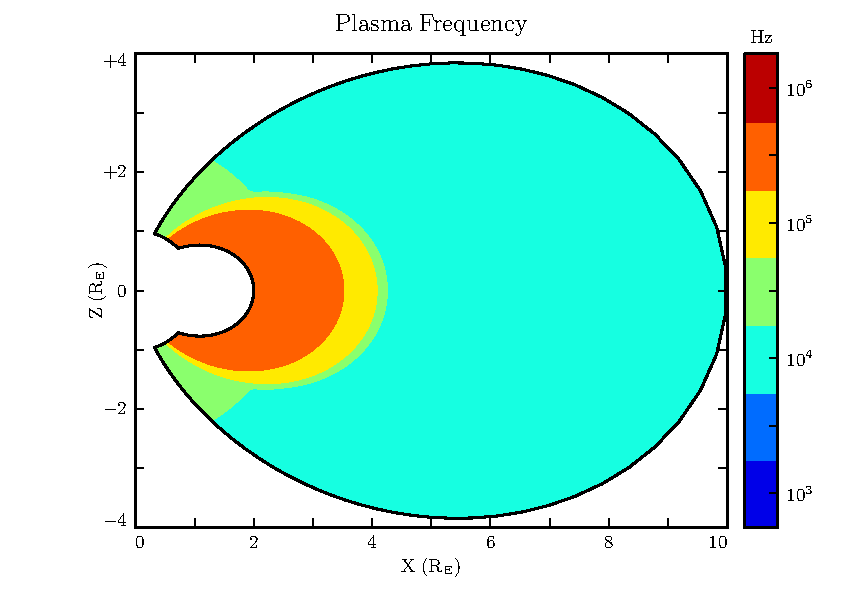
\includegraphics[width=\textwidth]{figures/op.pdf}
    \caption[Plasma Frequency Profile]{
      The plasma frequency reaches a peak value just under \SI{e7}{\radian/\second} near the equator. Outside the plasmasphere, its value is closer to \SI{e4}{\radian/\second}.  
    }
    \label{fig_op}
\end{figure}


%\todo{Generalized \ohmlaw, in case we decide we need it. Could talk through why all of the other terms are OK to neglect.  
%\begin{align}
%  \vec{E} + \cross{U}{B} & = 
%  \eta \vec{J} + \tfrac{\me}{n e^2} \lrb{
%    \tfrac{\partial}{\partial t} \vec{J} + \nabla \cdot \lr{ 
%      \vec{J} \, \vec{U} + \vec{U} \,\vec{J} +
%      \tfrac{1}{n e} \vec{J} \, \vec{J} } } +
%  \tfrac{1}{n e} \cross{J}{B} -
%  \tfrac{1}{n e} \div{ \vec{P_e} }
%\end{align}
%}

% -----------------------------------------------------------------------------
% -----------------------------------------------------------------------------
% -----------------------------------------------------------------------------
\subsection{Parallel Electric Fields}
  \label{sec_inertia_fields}





\todo{How much does electron inertia matter? }

\todo{Note, again, that only the figures in the present chapter include electron inertia. Those in \cref{ch_azm,ch_rbsp} do not, for the sake of stability and computational cost. }

\todo{Integrate up a parallel electric field to see the potential difference. Compare to the relation seen by \cite{olsson_1996}, $J_\parallel \sim \Psi_\parallel$ by a proportionality constant of \SIrange{e-8}{e-10}{\S/\meter\squared}. }

\todo{Parallel electric fields, supposedly, only appear at high altitude. \cite{marklund_1997,carlson_1998}. }





\todo{Even side-by-side, the magnetic fields in an otherwise-identical run are not visibly affected by the addition of electron inertial effects. }

%\begin{figure}[H]
%    \centering
%    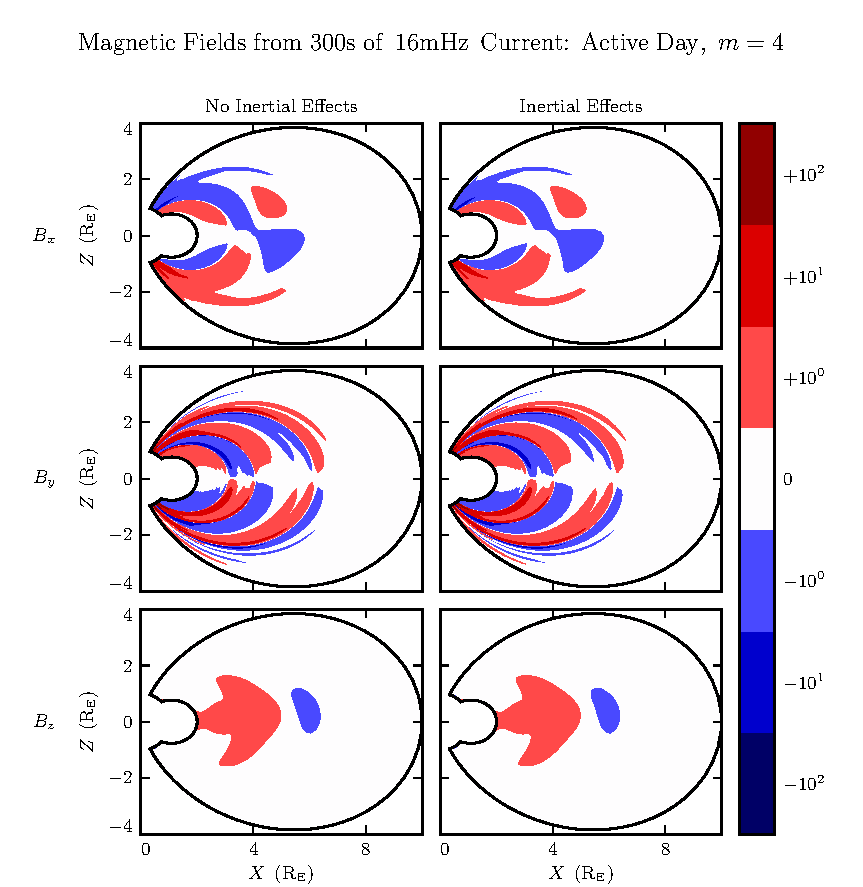
\includegraphics[width=\textwidth]{figures/B_1_004_016mHz.pdf}
%    \caption[Magnetic Fields With and Without Electron Inertia]{
%      The addition of electron inertial effects, with no other changes to the model, does not visible change the output. In a way, this is reassuring, since the alternative is to cast doubt on past work. 
%    }
%    \label{fig_B_1_004_016mHz}
%\end{figure}

\todo{The parallel electric fields do a bit better... after all, any change is a big change compared to zero. But they're still very small. }

With a bit of algebra, the meridional components of the dispersion tensor from \cref{sec_high_alt} provide a comparison of the parallel and perpendicular electric field magnitudes.
\begin{align}
  \frac{E_\parallel}{E_\bot} &= \frac{- k_\parallel k_\bot c^2 }{ \omega^2 - k_\bot^2 c^2 - \op^2 } \sim \frac{k^2 c^2 }{\op^2}
\end{align}

The electron inertial length $\frac{c}{\op}$ is on the order of \SI{1}{\km}, smaller than the wavelength of a field line resonance by three or four orders of magnitude. That is, at high altitude, the parallel electric field is expected to be smaller than the perpendicular electric field by a factor of \num{e7} -- perhaps more, depending on how closely the wave vector is aligned to the magnetic field. That seems fine -- note that \cref{fig_E_2_016_010mHz} shows that max $E_\parallel$ is 4 to 5 orders larger than max $E_\bot$... plus high altitude is the parallel field's minimum and the perpendicular field's maximum. 

\begin{figure}[H]
    \centering
    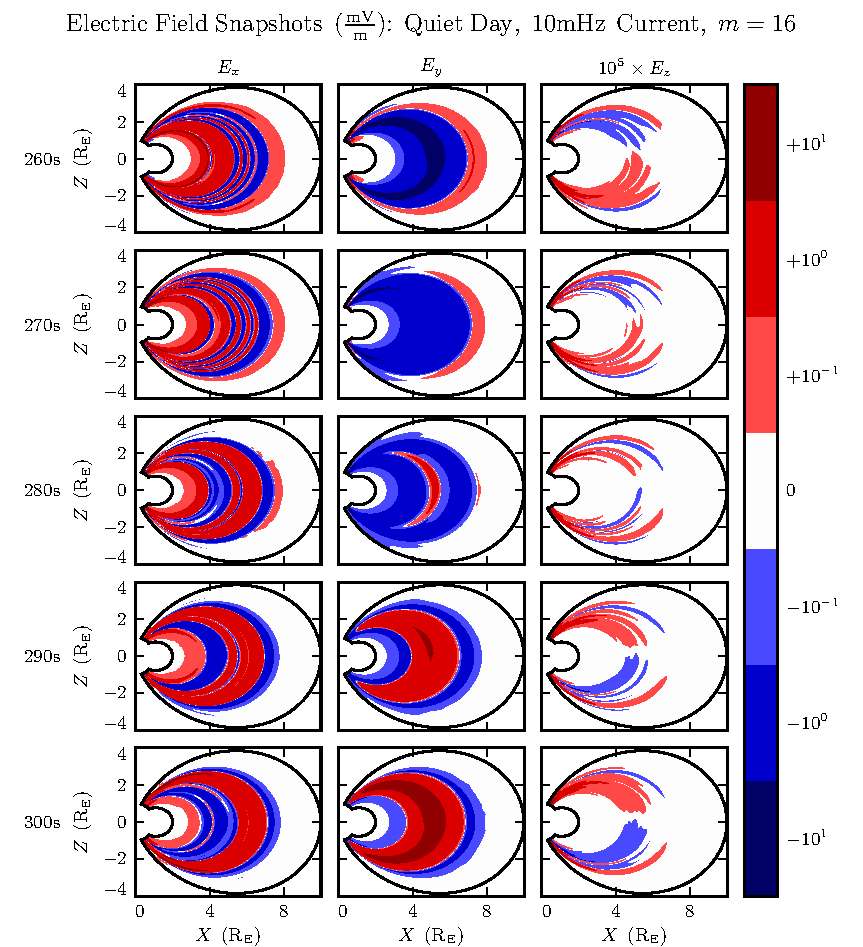
\includegraphics[width=\textwidth]{figures/E_2_016_010mHz.pdf}
    \caption[Parallel Electric Field Snapshots]{
      Parallel electric fields are smaller than perpendicular electric fields by at least four orders of magnitude.
    }
    \label{fig_E_2_016_010mHz}
\end{figure}

% -----------------------------------------------------------------------------
% -----------------------------------------------------------------------------
% -----------------------------------------------------------------------------
\subsection{Field-Aligned Current}
  \label{sec_fac}

\todo{The field-aligned current activity lines up with the Poynting flux. Poloidal Poynting flux is calculated from real $E_y$ and $B_x$. Toroidal Poynting flux is imaginary $E_x$ and $B_y$. The real component of the field-aligned current matches up with the poloidal, and the imaginary component lines up with the toroidal. }

\todo{Over the bulk of the simulation, each field is overwhelmingly either real or imaginary. However, that gets muddled at the ionosphere by the Hall conductivity (rather than being purely a function of azimuthal derivatives). }

\begin{figure}[H]
    \centering
    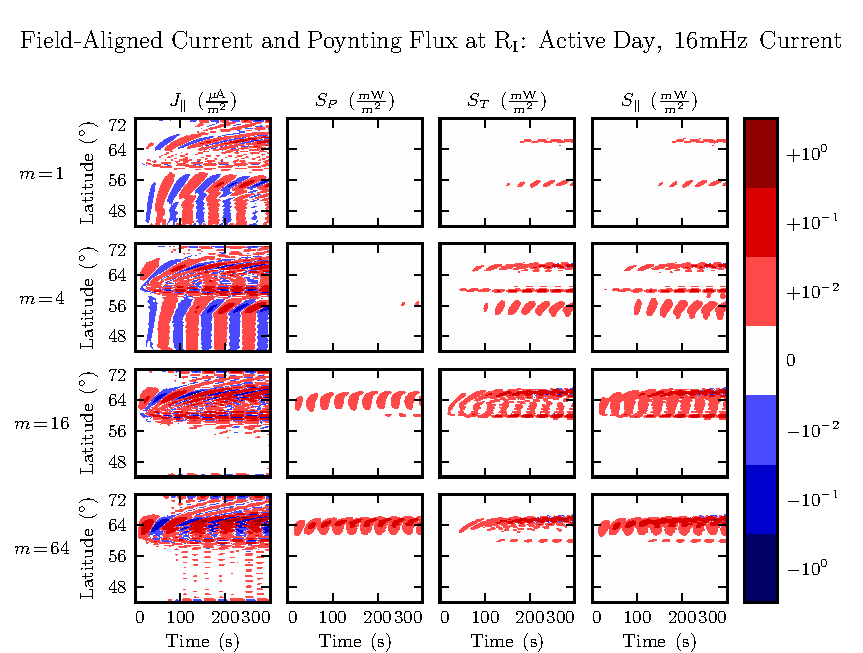
\includegraphics[width=\textwidth]{figures/JS_1_016mHz.pdf}
    \caption[Field-Aligned Current and Poynting Flux at the Ionosphere]{
      Perhaps unsurprisingly, field-aligned current structures at the ionospheric boundary line up with Poynting flux structures. The imaginary component of the current lines up with the toroidal Poynting flux (which is the product of imaginary $E_x$ and imaginary $B_y$), while the real current lines up with the poloidal Poynting flux ($E_y$ and $B_x$ are real). 
    }
    \label{fig_JS_1_016mHz}
\end{figure}

\todo{Notably, while the net Poynting flux is downward almost everywhere, field-aligned currents alternate between upward and downward flow. Perhaps this has to do with Poynting flux being a quadratic quantity while current is linear? }

The ``wigglies'' visible in the lower-left corner of \cref{fig_JS_1_016mHz} suggests overcorrection due to an improperly-coarse grid. See \cref{sec_lengths}. 

\todo{Field-aligned currents can be of significant size, but they're not particularly good at depositing energy in the ionosphere. As would be expected from energy conservation, $\nabla \cdot \vec{S}$ closely resembles $\vec{J} \cdot \vec{E}$, but only a vanishingly small portion of that is due to $J_z E_z$. }

\begin{figure}[H]
    \centering
    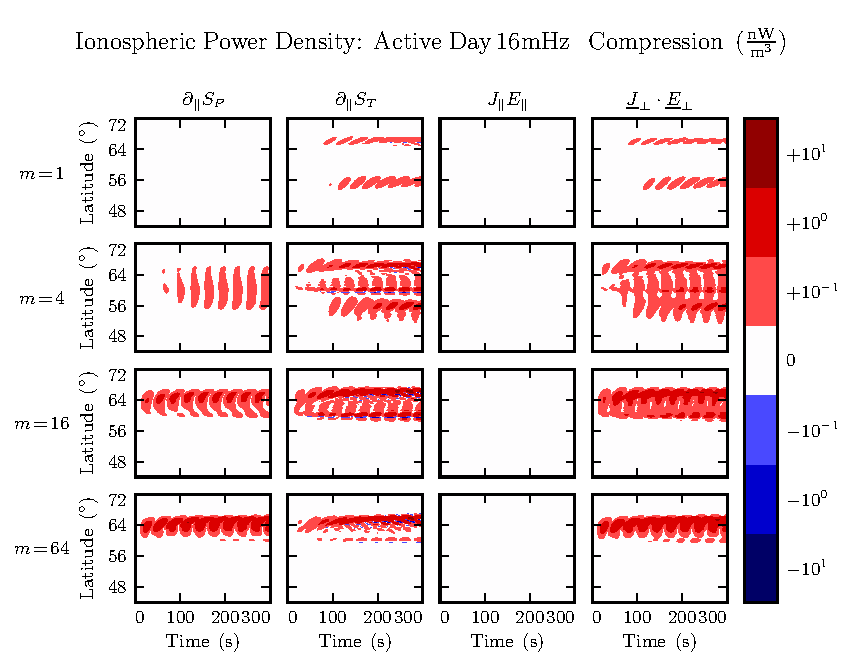
\includegraphics[width=\textwidth]{figures/JE_1_016mHz.pdf}
    \caption[Ionospheric Power Density]{
      While field-aligned currents can be of significant size, they are not particularly good at depositing energy in the ionosphere. Energy deposited by the Poynting flux matches closely with Joule dissipation from the perpendicular currents -- energy conservation! -- while $J_\parallel E_\parallel$ is smaller by several orders of magnitude. 
    }
    \label{fig_JE_1_016mHz}
\end{figure}

% -----------------------------------------------------------------------------
% -----------------------------------------------------------------------------
% -----------------------------------------------------------------------------
\subsection{Inertial Length Scales}
  \label{sec_lengths}

\todo{Are we really computing the electric fields faithfully? As touched on in \cref{sec_inertia_fields}, the perpendicular wavelength is important for determining the strength of the parallel electric field. This is because everything depends on derivatives, not magnitudes. }

\todo{A typical run has maximum perpendicular electric field on the order of \SI{10}{\mV/\meter}. Maybe a bit more. Field structures vary on the order of as little as $\sim\SI{1}{\degree}$. That could give up to $\curl{E} \sim \SI{e2}{nT/\second}$. In comparison parallel electric fields max out around \SI{e-3}{\mV/\meter}. If that varies as a scale of the inertial length -- as we expect, recalling \cref{sec_boris} -- that's order of \SI{1}{\km}, it could give $\curl{E} \sim \SI{1}{nT/\second}$. Plausibly large enough to have a visible effect. Note that the electron inertial length only needs to be resolved in the perpendicular direction, since that's where we're taking curls of the parallel electric field... which is the only quantity expected to change significantly (to lowest order) as a result of electron inertial effects. }

\todo{This poses a significant computational cost. Within the plasmasphere, the inertial length is on the order of \SI{0.1}{\km}. That's two-plus orders of magnitude smaller than the present grid. Moving the inner boundary from $L=2$ to $L=5$ makes up half of that. }

\todo{We do a few runs which sorta resolve the electron inertial length. It's about \SI{2}{\km}, and we get resolution down to \SI{0.7}{\km}. This is a factor of ten increase in resolution, and an additional factor of ten decrease in the time step (due to the drop in \Alfven crossing time). It's not enough. \cref{fig_Ez_inertial_length} is clearly not well-resolved. Those wigglies are probably about to cause a crash. }

\begin{figure}[H]
    \centering
    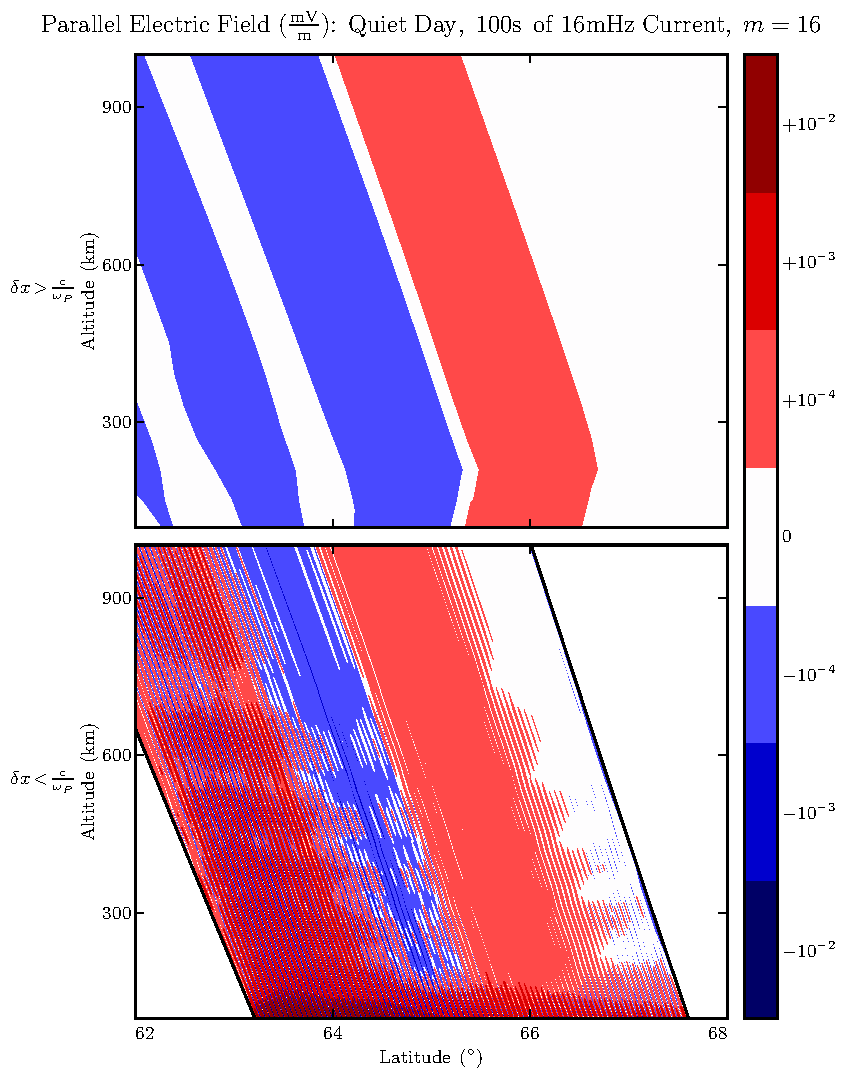
\includegraphics[width=\textwidth]{figures/Ez_inertial_length.pdf}
    \caption[Parallel Electric Fields by Perpendicular Grid Resolution]{
      The parallel electric field develops significant structure when the perpendicular grid resolution is smaller than the electron inertial length. Unfortunately, such runs are prohibitively expensive. The lower panel -- which still fails to resolve wave structure properly -- represents a 100-fold increase in computational time. 
    }
    \label{fig_Ez_inertial_length}
\end{figure}

\todo{The moral of the present section is that proper handling of electron inertial effects will probably show additional structure at small scales... but that simulating those structures is computationally expensive in terms of computational expense, even in 2.5D. }




% %%%%%%%%%%%%%%%%%%%%%%%%%%%%%%%%%%%%%%%%%%%%%%%%%%%%%%%%%%%%%%%%%%%%%%%%%%%%%
% %%%%%%%%%%%%%%%%%%%%%%%%%%%%%%%%%%%%%%%%%%%%%%%%%%%%%%% Building on Mann 1995
% %%%%%%%%%%%%%%%%%%%%%%%%%%%%%%%%%%%%%%%%%%%%%%%%%%%%%%%%%%%%%%%%%%%%%%%%%%%%%

\chapter{Results}
  \label{ch_results}

\todo{This chapter is the real moneymaker. The overarching motivation for this work is that Pc4 pulsations vary in interesting ways with respect to azimuthal modenumber, and that prior models have been unable to give a good picture of that behavior. }

%\todo{Do we every check E/B against $\Sigma_P / \mz$? }

%\todo{Do we see a difference between \vec{k} (momentum) and the group velocity? Poynting flux will always be pretty much along the field line, since $B_3$ is small and $E_3$ is zero, but the wave vector need not be. This is a question of coupling/converting to compressional waves, I guess. }

%\todo{Look at McKenzie and Westphal. Waves incident on the bow shock, etc, at weird angles. }

%\todo{Look at the E to B ratio. Compare to the \Alfven speed and to the height-integrated Pedersen conductivity. }

% =============================================================================
% =============================================================================
% =============================================================================
%\section{Electromagnetic Energy Gap}

%\todo{A preliminary search (and asking Bob) has not turned up anyone looking at this before, so it's hard to provide context. }

%Above, we considered the decay of energy from the poloidal mode to the toroidal mode. A natural follow up is, are there any other surprising trends in the distribution of energy?

%As it turns out, yes!

%In cases where the driving frequency does not line up with the local bounce frequency, energy doesn't accumulate particularly well in either the poloidal or the toroidal mode. Like a damped-driven oscillator, the system's behavior follows the input. 

%At low \azm, what energy there is divides itself more or less equally between the electric and magnetic fields. 

%As \azm increases, oddly, a gap appears. When the conductivity is high, the magnetic field holds more energy than the electric field. The disparity can be up to a factor of $\sim \num{3}$; that is, \SI{75}{\percent}. of the energy in the magnetic field, and \SI{25}{\percent} in the electric field. When conductivity is low, the opposite happens: energy concentrates in the electric field. 

%This lines up somewhat with what might be expected. When conductivity is low, it takes a larger electric field to induce the same current, and thus the same magnetic field. But it's not clear why this disparity only appears at large \azm, or why it does not appear when the driving is resonant. 

%Maybe it's a timing issue? A relationship between the bounce time (which is more or less indepedent of \azm) and the rotation time (which depends on \azm). 

%\todo{How is the compressional magnetic field brought into these calculations? It exists only at small \azm. It's never particularly large, it also gets added to the zeroth-order field before squaring. }

%\begin{figure}[H]
%    \centering
%    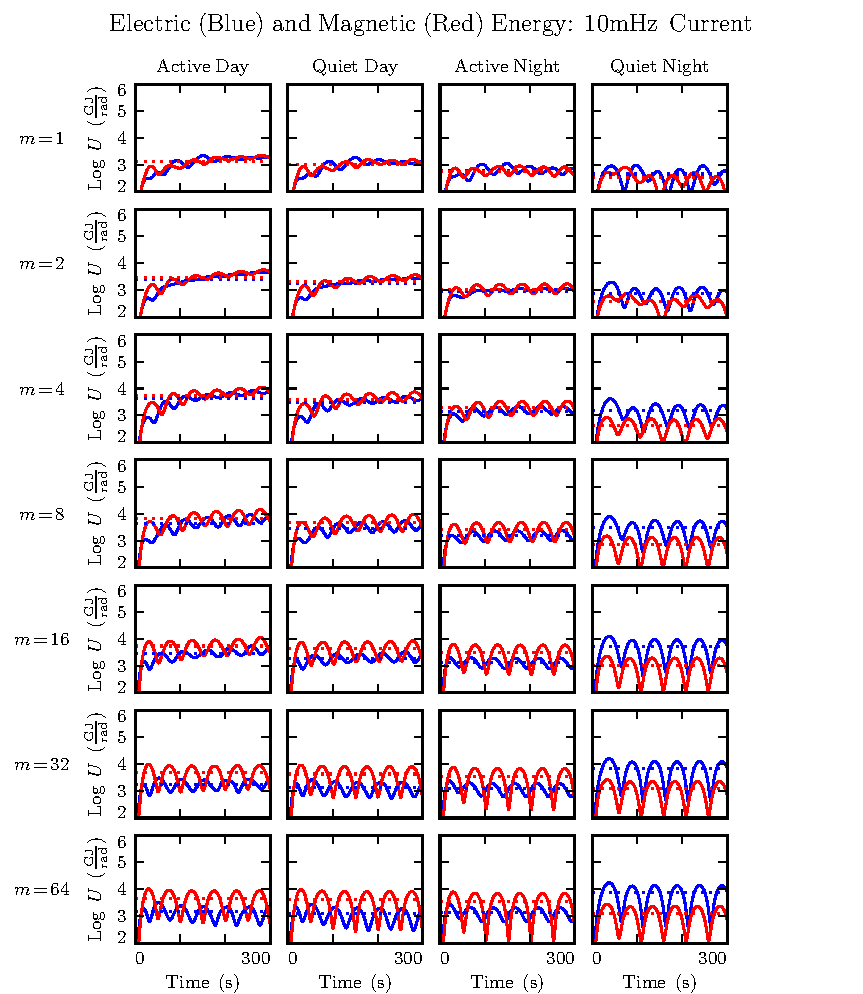
\includegraphics[width=\textwidth]{figures/U_BE_010mHz.pdf}
%    \caption[Current-Driven Electric and Magnetic Energy: 10mHz]{
%      In the absence of resonant driving, a disparity emerges at large \azm between the energy in the magnetic field and the energy in the electric field. The sign of the difference depends on the ionospheric conductivity. 
%    }
%    \label{fig_U_BE_010mHz}
%\end{figure}

%\begin{figure}[H]
%    \centering
%    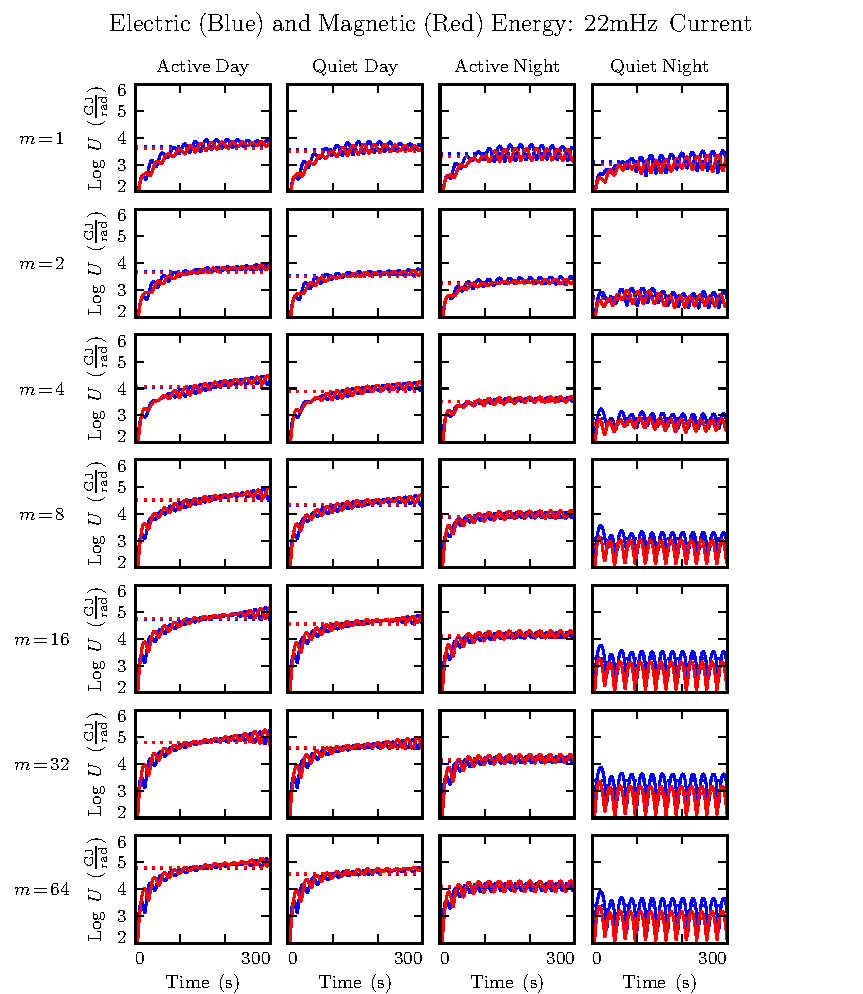
\includegraphics[width=\textwidth]{figures/U_BE_022mHz.pdf}
%    \caption[Current-Driven Electric and Magnetic Energy: 22mHz]{
%      When driving is resonant, energy is distributed almost exactly half-and-half between the electric and magnetic fields, regardless of \azm. The rightmost profile still shows a gap, likely because the ionospheric conductivity in that model is low enough that nothing ever resonates. 
%    }
%    \label{fig_U_BE_022mHz}
%\end{figure}













  
% =============================================================================
% =============================================================================
% =============================================================================
\section{Finite Poloidal Lifetimes}
  \label{sec_lifetimes}

Radoski\cite{radoski_1974} looked at \Alfven waves, using a cylindrical coordinate system to imitate an ``unwrapped'' dipole. He argued that poloidal waves should asymptotically rotate to the toroidal mode. 

Mann\cite{mann_1995} performed some wave-in-a-box simulations and found the rotation time to be linear in modenumber: $\tau = \frac{d \lambda}{d \omega_A'}$, where $\lambda = \frac{\azm}{2 \pi r}$ and $\omega_A'$ is the spatial derivative of the \Alfven bounce frequency. Soon afterwards\cite{mann_1997}, he supported his simulations analytically. 

\todo{Crunch out $\frac{d \lambda}{d \omega_A'}$. Preliminary indications are that it doesn't translate well to a realistic grid, but let's double check. }

Ding\cite{ding_1995} ran simulations more-or-less concurrent with Mann's. Ding saw a rotation from poloidal to toroidal... then back again. It seems that the reversal was a spatial resolution issue. 

The aforementioned models made significant simplifying assumptions in terms of geometry and boundary conditions. 

Mann used straight field lines, a uniform \Alfven speed gradient, and perfectly conducting boundaries. 

Ding's simulation is nominally carried out in a dipole geometry, but the ionospheric boundary is at \SI{2.5}{\RE}. Boundaries are also perfectly conducting. 

That is, the results below offer a significantly higher level of realism than any past simulation (in part, of course, because computers are a lot better than they were 20 years ago). 

A dedicated 3D treatment of this problem is unlikely at present. Large azimuthal modenumbers are expensive to compute. That's the whole point! 

The energy is obtained by integrating (using the Jacobian to handle the grid properly) $U = \int dU = \int u \, dV$. Values are the log (base 10) of that, in the slightly odd units of gigajoules per radian. A factor of $2\pi$ wouldn't change anything, of course, but it seems inappropriate to integrate all the way around the sphere when Pc4s are longitudinally localized (a fact which was an important part of justifying a 2.5D approach). 

% -----------------------------------------------------------------------------
% -----------------------------------------------------------------------------
% -----------------------------------------------------------------------------
\subsection{High Conductivity}

In \cref{fig_U_day}, the rotation of energy from the poloidal mode to the toroidal mode is clear. Driving is strictly poloidal, yet the toroidal mode accumulates energy over time, and doesn't appear to give it back. The rotation happens faster for low-\azm simulations, qualitatively consistent with Mann's result; the time at which poloidal and toroidal energies are equal seems to even be linear in \azm, in line with his result. 

At least, this is the case on the dayside, where the ionosphere is highly conductive. 

\begin{figure}[H]
    \centering
    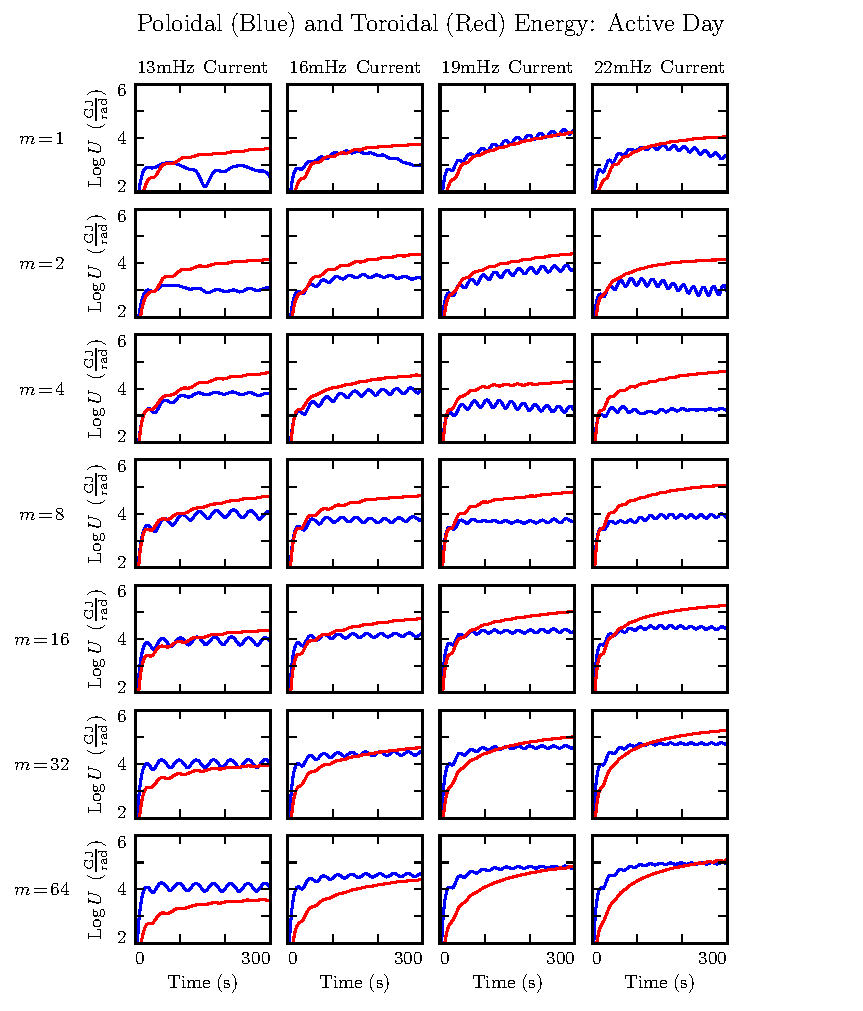
\includegraphics[width=\textwidth]{figures/U_1.pdf}
    \caption[Poloidal and Toroidal Energy: Active Day]{
      Driving -- delivered to the poloidal mode -- asymptotically rotates to the toroidal mode. The rate of rotation is strongly affected by the azimuthal modenumber. 
    }
    \label{fig_U_day}
\end{figure}

\todo{Talk about why this is exciting. }

\todo{Note that Mann looked specifically at second-harmonic waves. }

\todo{This result shows agreement with -- and significant refinement of -- Mann's findings. In the case of large-but-finite ionospheric conductivity, dipole geometry, and realistic \Alfven speed profile, energy does asymptotically rotate from the poloidal mode to the toroidal mode. The rotation rate is strongly affected by azimuthal modenumber and, in the case of large-but-finite \azm, has a characteristic timescale in the tens of periods. The present work furthermore demonstrates that the rotation rate is affected by driving frequency (did Mann talk about this at all, or just work in normalized time?) }

% -----------------------------------------------------------------------------
% -----------------------------------------------------------------------------
% -----------------------------------------------------------------------------
\subsection{Low Conductivity}

The picture on the nightside (where the ionospheric conductivity is low) is significantly different from the dayside (where it's high). 

Dissipation seems to outstrip rotation. Energy does not accumulate over numerous driving periods, as would be expected in resonance; it follows the driving up and down, as a damped-driven oscillator. 

There is evidence that the rotation is still trying to happen. At low \azm, energy is distributed between the poloidal and toroidal mode before dissipating; at high \azm, the energy dissipates straight out of the poloidal mode, never having had a chance to rotate. 

\begin{figure}[H]
    \centering
    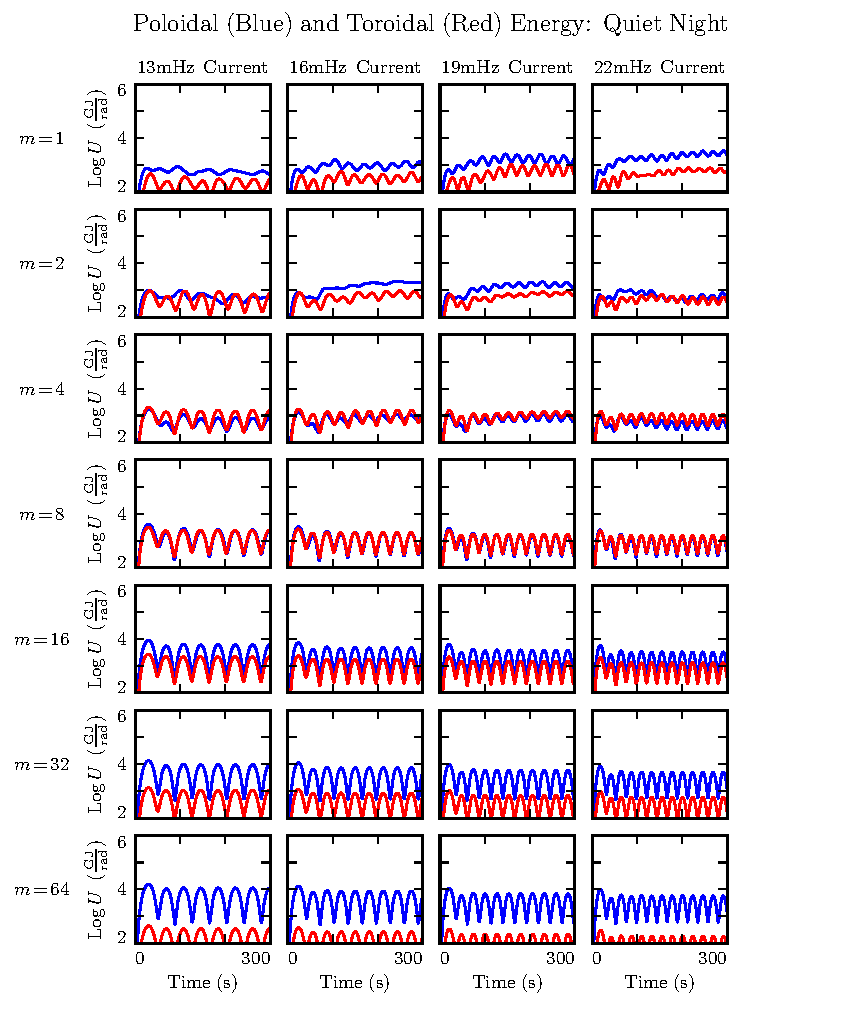
\includegraphics[width=\textwidth]{figures/U_4.pdf}
    \caption[Poloidal and Toroidal Energy: Quiet Night]{
      Driving is applied to the poloidal electric field. There is some rotation of energy to the toroidal mode (and less at high azimuthal modenumber), but the low ionospheric conductivity prevents energy from accumulating over time. 
    }
    \label{fig_U_night}
\end{figure}

\todo{Why is this exciting? }

\todo{Previous considerations of poloidal lifetimes have been limited to the high conductivity regime. The present work demonstrates that the low conductivity regime exhibits qualitative differences. Ionospheric conductivity on the nightside is low enough that resonance does not develop, even in the case of ongoing driving. The dissipation timescale is comparable to the rotation timescale. Rather than aymoptotically accumulating energy in the toroidal mode, the oscillator asymptotically oscillates following the driving. This is relevant to the question of day-night asymmetry in the observation of field line resonances. }


  
% =============================================================================
% =============================================================================
% =============================================================================
\section{Spatial Distribution of Energy}
  \label{sec_shells}

Looking a bit deeper, it's possible to comment on the structure of the poloidal and toroidal modes, not just their magnitudes. The following commentary addresses the dayside; on the nightside, there's never much by the way of resonance. 

In \cref{fig_resonant_driving,fig_nonresonant_driving}, electromagnetic energy is binned by field line, averaged over volume (again, with respect to the Jacobian), and plotted as contours. All plots share a color scale. 

The poloidal mode and the toroidal mode exhibit qualitatively different behavior, related to the fact that energy rotates from poloidal to toroidal, and not back. 

At low \azm, energy rotates out of the poloidal mode so quickly that no resonance can form. 

At high \azm, the \Alfven wave is guided. If the driving frequency lines up with the resonant frequency where it's delivered, the poloidal mode resonates strongly. Otherwise, again, no energy accumulates. 

In no case does the poloidal mode demonstrate the ability to move energy across magnetic field lines. 

On the other hand, the toroidal mode does resonate, even if the driving isn't resonant (though in that case the response is of course stronger). The toroidal mode transports energy across field lines until it encounters resonance, then accumulates energy there. Often, resonances are seen in multiple locations due to the non-monotonic \Alfven bounce frequency (recall \cref{fig_fa}) as a function of $L$. 

% -----------------------------------------------------------------------------
% -----------------------------------------------------------------------------
% -----------------------------------------------------------------------------
\subsection{Resonant Driving}

\begin{figure}[H]
    \centering
    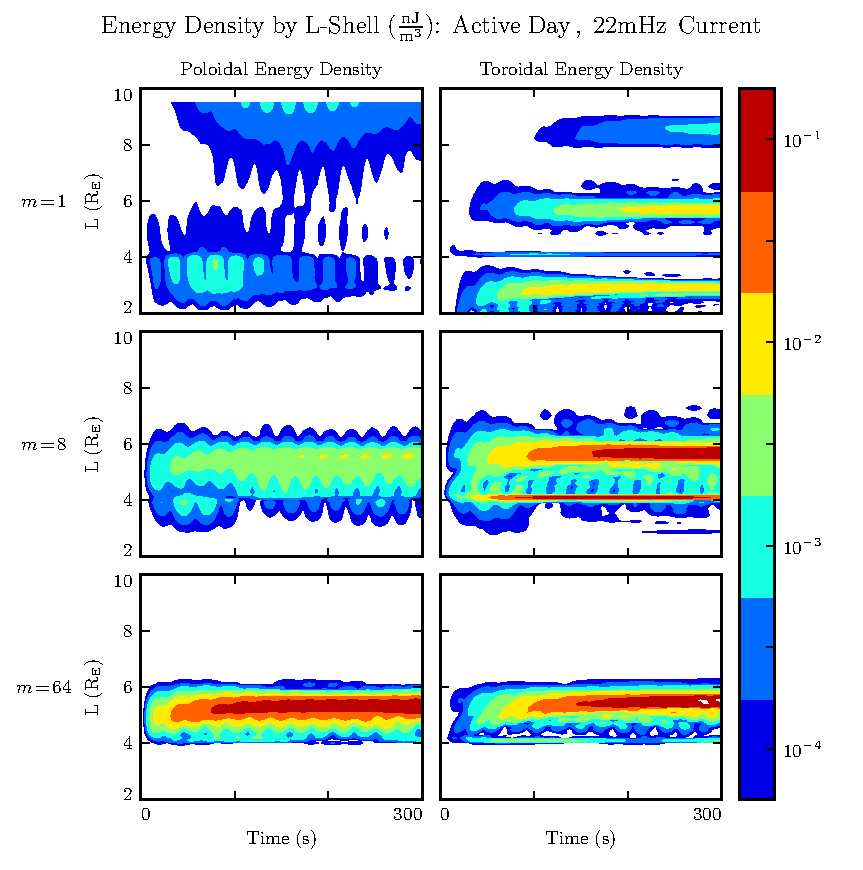
\includegraphics[width=\textwidth]{figures/layers_22mHz_1.pdf}
    \caption[Poloidal and Toroidal Energy Distribution: Resonant Driving]{
      If \azm is small, energy rotates to the toroidal mode too fast to form a poloidal resonance. If \azm is large, the \Alfven wave is guided, so it resonates only if the driving frequency lines up with the resonant frequency where it's applied. The result is just one big -- or perhaps even giant -- pulsation. If the driving lines up with a nearby field line, the toroidal mode goes crazy! Resonance inside the plasmasphere. Resonance at the plasmapause. Resonance at the driving location. And (weak) attempt at a higher harmonic further out. 
    }
    \label{fig_resonant_driving}
\end{figure}

\todo{Why is this exciting? }

\todo{Driving from inside the magnetosphere is novel. }

% -----------------------------------------------------------------------------
% -----------------------------------------------------------------------------
% -----------------------------------------------------------------------------
\subsection{Nonresonant Driving}

\begin{figure}[H]
    \centering
    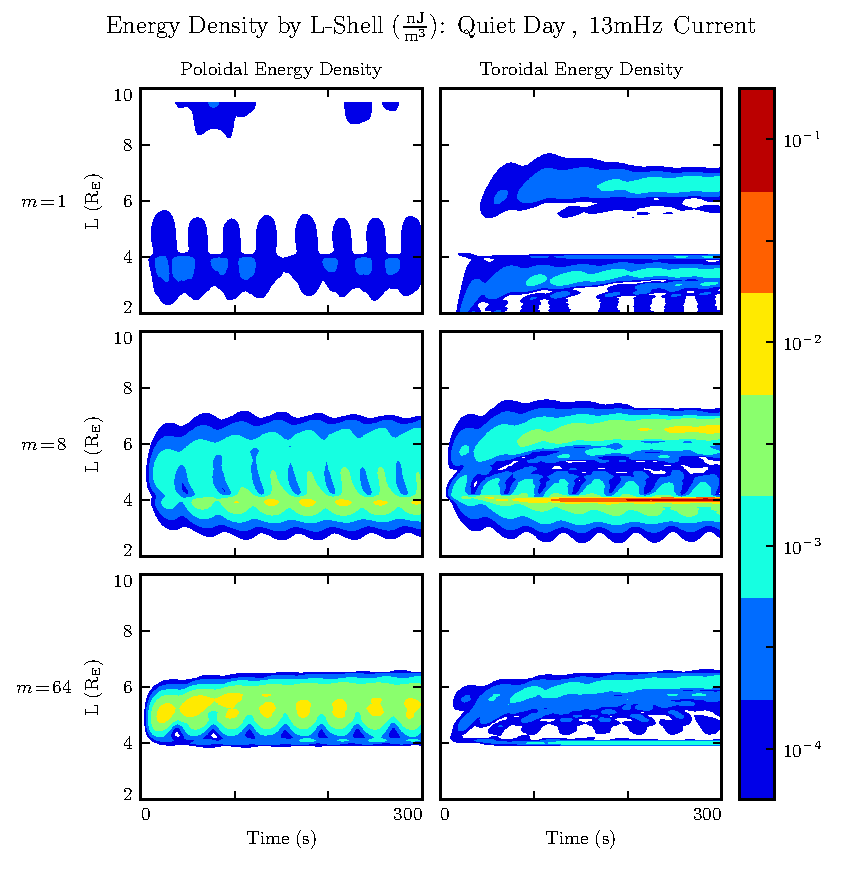
\includegraphics[width=\textwidth]{figures/layers_13mHz_2.pdf}
    \caption[Poloidal and Toroidal Energy Distribution: Nonresonant Driving]{
      When the driving frequency doesn't line up with the location where it's delivered, there's basically no response. There is no movement of energy to a resonant field line, so no energy can accumulate over the course of multiple rounds of driving. Even when not driven resonantly, the toroidal mode still makes the best of its situation. It steals what energy it can from the poloidal mode, carries it to the resonant $L$-shell, and gets to work. (In contrast, recall from \cref{fig_resonant_driving}, in this situation the poloidal mode just does not accumulate energy.)
    }
    \label{fig_nonresonant_driving}
\end{figure}

\todo{Why is this exciting? }


  
% =============================================================================
% =============================================================================
% =============================================================================
\section{Significance for Giant Pulsations}

Giant pulsations are (probably\cite{takahashi_2011}) fundamental mode poloidal Pc4 pulsations with frequencies around \SI{10}{\mHz} and azimuthal modenumbers around \num{20}. They are large, and can sometimes be observed on the ground. 

While this model makes no particular distinction between a giant pulsation and any other Pc4, the above results do line up with giant pulsation observations. 

Giant pulsations aren't seen at small \azm. As shown in \cref{sec_lifetimes}, low-\azm poloidal modes rotate to the toroidal mode too quickly to resonate effectively, even in the case of continuous driving at a locally-resonant frequency. The sweet spot seems to be around $\azm = 20$, more or less the same point where resonance becomes visible in \cref{fig_resonant_driving}. Admittedly, giant pulsations are typically closer to \SI{10}{\mHz} than \SI{22}{\mHz}. It seems likely that qualitatively similar results would be encountered if the driving were moved to an $L$-shell with a bounce time of \SI{10}{\mHz}. 

% -----------------------------------------------------------------------------
% -----------------------------------------------------------------------------
% -----------------------------------------------------------------------------
\subsection{Ground Signatures}

\todo{\cite{takahashi_2011} talks significantly about the east-west polarization. }

Giant pulsations are seen at very large \azm, though not on the ground\cite{takahashi_2013}, due to damping by the ionosphere. 

Giant pulsations are most common on the dayside (particularly the morningside), during geomagnetically quiet times. Giant pulsation ground signatures are noted for their predisposition towards east-west polarization. 

In \cref{fig_ground_signatures}, the strongest east-west ground signatures is obtained on the geomagnetically quiet dayside, at \azm of 16 and 32. 

This seems to be a giant pulsation ``sweet spot'': the poloidal mode becomes stronger as \azm increases, but the ionospheric damping also increases. 

\begin{figure}[H]
    \centering
    \includegraphics[width=\textwidth]{figures/ground_16mHz.pdf}
    \caption[Dayside Ground Magnetic Fields]{
      The east-west component of magnetic ground signatures is peaked on the geomagnetically quiet dayside, at modenumbers around 16 to 32. This coincides nicely with observations of giant pulsations. Like the east-west component, the north-south ground signature is strongest on the quiet dayside; however, unlike the east-west component, the north-south component is weak when the modenumber is large. 
    }
    \label{fig_ground_signatures}
\end{figure}

Giant pulsations are monochromatic, and can be accompanied by ``multiharmonic toroidal waves''\cite{takahashi_2011}. Per \cref{sec_shells}, this is about what would be expected from a mishmash of poloidal driving. Poloidal modes of all frequencies rotate into the toroidal mode; resonant poloidal modes resonate; non-resonant poloidal modes become evanescent. 

Giant pulsations often drift azimuthally. This model can't resolve azimuthal drift directly, of course, but can fake it by looking at complex phase. There has been some indication (not shown) of complex phase rotation in ground magnetic fields. However, at the boundary, it's difficult to disentangle which values are imaginary to indicate an azimuthal offset, and which are imaginary because of Hall coupling. Investigation is ongoing. 




% %%%%%%%%%%%%%%%%%%%%%%%%%%%%%%%%%%%%%%%%%%%%%%%%%%%%%%%%%%%%%%%%%%%%%%%%%%%%%
% %%%%%%%%%%%%%%%%%%%%%%%%%%%%%%%%%%%%%%%%%%%%% Validate the Model Against RBSP
% %%%%%%%%%%%%%%%%%%%%%%%%%%%%%%%%%%%%%%%%%%%%%%%%%%%%%%%%%%%%%%%%%%%%%%%%%%%%%

\chapter{Observations}
  \label{ch_rbsp}

\todo{Do we need to acknowledge that a moving spacecraft might have these fields shifted per $\vec{E} + \cross{U}{B}=0$? }

\todo{I have met a handful of times with John (Wygant) to discuss how to get some RBSP data into this dissertation.}

\todo{John has recently become interested in the long (\SI{26}{\day} or so) cycle in the size of the plasmapause.}

\todo{Lei recently compiled a list of several hundred Pc4 events seen by RBSP\cite{dai_2015}. He binned them by plasmapause location, noting that there were a significant number of events in the entire interval $4 \lesssim L \lesssim 6$. However, he was just writing about occurrence rate, so he didn't delve into how the large-plasmasphere Pc4s were different from the small-plasmasphere ones.}

\todo{I'll bet I can find a pattern or two in Pc4 behavior based on plasmapause location. It'll be interesting to see if the model exhibits the same pattern as the plasmapause location is adjusted.}

\todo{I emailed Lei about this earlier this week. He sent over his event list.}

\todo{Sheng has agreed to show me how to access RBSP data.}

\todo{There is some concern about the rules attached to funding. Apparently NASA fundees aren't allowed to be involved in two-person collaborations with international scientists, or something? We'll have to get that figured out. }

% =============================================================================
% =============================================================================
% =============================================================================
\section{Event Selection}

% -----------------------------------------------------------------------------
% -----------------------------------------------------------------------------
% -----------------------------------------------------------------------------
\subsection{Identifying the Fundamental Harmonic}

Takahashi\cite{takahashi_2013} spells this out explicitly. Fundamental mode, south of the equator, V should lead B by 90 degrees. 

Per Takahashi\cite{takahashi_2011}, phase lag can be used to distinguish the fundamental harmonic from the second harmonic. 

Chisham and Orr\cite{chisham_1991} argue that around \SI{7}{\RE}, frequency around \SI{10}{\mHz} precludes higher harmonics. Or maybe look at \cite{green_1985}?

Green\cite{green_1979} and Cummings\cite{cummings_1969} talk about the frequencies for ideal toroidal modes. 

Dai\cite{dai_2015} says to look at \cite{takahashi_2011} and \cite{dai_2013} for unambiguous identification of the fundamental mode. 

% =============================================================================
% =============================================================================
% =============================================================================
\section{Something Something Results}

% -----------------------------------------------------------------------------
% -----------------------------------------------------------------------------
% -----------------------------------------------------------------------------
\subsection{Something Something Results}










  
% =============================================================================
% =============================================================================
% =============================================================================
\section{Event Selection}




Note that, in gathering his 860 events, Dai\cite{dai_2015} did not take the $\vec{E} \cdot \vec{B} = 0$ assumption to clean up the electric field data. The present work has taken that assumption -- and discarded all events within \SI{15}{\degree} of the probe's spin axis. 

This cuts it down to ... events. 

Furthermore distinguish the fundamental mode from the second harmonic...

Insist on a certain confidence... 



% -----------------------------------------------------------------------------
% -----------------------------------------------------------------------------
% -----------------------------------------------------------------------------
\subsection{Identifying the Fundamental Harmonic}

Takahashi\cite{takahashi_2013} spells this out explicitly. Fundamental mode, south of the equator, V should lead B by 90 degrees. 

Per Takahashi\cite{takahashi_2011}, phase lag can be used to distinguish the fundamental harmonic from the second harmonic. 

Chisham and Orr\cite{chisham_1991} argue that around \SI{7}{\RE}, frequency around \SI{10}{\mHz} precludes higher harmonics. Or maybe look at \cite{green_1985}?

Green\cite{green_1979} and Cummings\cite{cummings_1969} talk about the frequencies for ideal toroidal modes. 

Dai\cite{dai_2015} says to look at \cite{takahashi_2011} and \cite{dai_2013} for unambiguous identification of the fundamental mode. 

\cite{liu_2010} talks about setting the coordinate system using the time-averaged magnetic field, and the azimuthal direction being $\hat{B_0} \times \hat{r}$. 


  
% =============================================================================
% =============================================================================
% =============================================================================
\section{Something Something Results}

Brekke\cite{brekke_1987} looked at 523 giant pulsation events recorded at Troms{\o}, Norway, from 1929 to 1985. This spanned several solar cycles. 

Rolf\cite{rolf_1931} collected 28 events between 1921 and 1930 at Abisko. 

Sucksdorf\cite{sucksdorf_1939} got 150 events between 1914 and 1938 in Sodankyl{\"a}. 

Harang\cite{harang_1941}. 97 events from 1929 to 1941. Also Troms{\o}. 

This comes out to ... events over ... years. That's about ... giant pulsations per year, observed on the ground. 

\todo{Note that it's a bit tricky to compare ground observations to in situ observations. Large-\azm events won't make it through the ionosphere. }

\todo{How strong does an event need to be on the ground, or in the sky, to count as a giant pulsation? }

These observations were all recorded at single points on the ground, with magnetic latitude near \SI{66}{\degree}. 

Velkamp\cite{veldkamp_1960} looked at a single large event and showed that, at best, it was visible over a span of \SI{5}{\degree} in magnetic latitude. This is consistent (?) with the 29 February 2012 event discussed in detail by Motoba\cite{motoba_2015}. 

If peak Pg observations are at $\SI{66}{\degree}$ mlat, that corresponds to $L = 6$. Then let's suppose that peak Pg viewing is $\SI{5}{\degree}$ wide -- estimating from the work of Velkamp and Motoba. That means RBSP should see lots of Pgs when it's between $L = 5.2$ andn $L = 7.1$. Well, \SI{7.1}{\RE} is outside its apogee, but the probes spend a fair amount of time outside $L = 5.2$, since they are moving pretty slowly at that point. 

In addition, there should be no bias between an orbiting satellite and a ground-based magnetometer. Dai's analysis was specifically chosen to take advantage of the fact that RBSP's orbit had precessed all the way around the Earth. No preferred direction. 

\todo{How much time does each RBSP probe spend outside $L = 5.2$? }

\todo{How many Pgs, then, should we expect to see? }

\todo{How many fundamental mode poloidal Pc4 events can we find? They don't need to be pretty. They do need to have clear spectra. }

\todo{If we relax the \SI{15}{\degree} assumption to, say, \SI{5}{\degree}, how many events do we get? If we assume the probe's spin axis is uncorrelated to the harmonic mode of the event (which it should be!) when how many events do we ``see''? }

\todo{How many events do we see that could pass for Pgs? Note that \cite{takahashi_2013} has shown that it's OK to call something a giant pulsation even if it doesn't have a ground signature. }

Motoba, in 2015, recorded 105 giant pulsation events. The observations were carried out by a number of ground magnetometers spanning $\sim \SI{90}{\degree}$ in local time and ranging roughly \SIrange{60}{70}{\degree} magnetic latitude\cite{motoba_2015}. 

Giant pulsations have been shown to be more numerous in times of low solar activity. That was the whole point of Brekke's seminal 1987 paper, and it's consistent with what we show in \cref{sec_pgs}. 

The RBSP observations occur during peak solar times, though it's an anemic solar peak\cite{pesnell_2016}. 

RBSP-A and RBSP-B count as two observers. In one $\sim 5$ cases out of hundreds do they simultaneously observe a poloidal Pc4 event (although, most notably for the 2012 event which \cite{dai_2013} considers in detail, both probes do fly through the same apparent event several hours apart from one another. 






% -----------------------------------------------------------------------------
% -----------------------------------------------------------------------------
% -----------------------------------------------------------------------------
\subsection{Something Something Results}





% %%%%%%%%%%%%%%%%%%%%%%%%%%%%%%%%%%%%%%%%%%%%%%%%%%%%%%%%%%%%%%%%%%%%%%%%%%%%%
% %%%%%%%%%%%%%%%%%%%%%%%%%%%%%%%%%%%%%%%%%%%%%%%%%%%%%%%%%%%%%%%%%% Conclusion
% %%%%%%%%%%%%%%%%%%%%%%%%%%%%%%%%%%%%%%%%%%%%%%%%%%%%%%%%%%%%%%%%%%%%%%%%%%%%%

\chapter{Conclusion}
  \label{ch_conclusion}

% =============================================================================
% =============================================================================
% =============================================================================
\section{Summary of Results}

\todo{Write this. }

% =============================================================================
% =============================================================================
% =============================================================================
\section{Future Work}

Arbitrary deformation of grid. Get $\hat{e}_i = \frac{\partial}{\partial u^i} \underline{x}$, then $g_{ij} = \hat{e}_i \cdot \hat{e}_j$, then invert the metric tensor for contravariant components.  

MPI. Some benchmarks with time to compute vs time to broadcast. At what problem scale does additional parallelization make sense? 

Driving based on events? Wouldn't be that hard. 

Test particles? Seems silly. Watching something drift-bounce resonate will require making assumptions about what's going on on the other face of the planet.  

Conductivity affected by precipitation/current? 

IRI ionosphere model. Solar illumination effects. 

  % =============================================================================
% =============================================================================
% =============================================================================
\section{Summary of Results}

\todo{Write this. }


  
% =============================================================================
% =============================================================================
% =============================================================================
\section{Future Work}

Arbitrary deformation of grid. Get $\hat{e}_i = \frac{\partial}{\partial u^i} \underline{x}$, then $g_{ij} = \hat{e}_i \cdot \hat{e}_j$, then invert the metric tensor for contravariant components.  

MPI. Some benchmarks with time to compute vs time to broadcast. At what problem scale does additional parallelization make sense? 

Driving based on events? Wouldn't be that hard. 

Test particles? Seems silly. Watching something drift-bounce resonate will require making assumptions about what's going on on the other face of the planet.  

Conductivity affected by precipitation/current? 

IRI ionosphere model. Solar illumination effects. 


% Bibliography
\bibliography{thesis}

% Appendices
\appendix

%%%%%%%%%%%%%%%%%%%%%%%%%%%%%%%%%%%%%%%%%%%%%%%%%%%%%%%%%%%%%%%%%%%%%%%%%%%%%%%%
% app_glossary.tex: Glossary Appendix:
%%%%%%%%%%%%%%%%%%%%%%%%%%%%%%%%%%%%%%%%%%%%%%%%%%%%%%%%%%%%%%%%%%%%%%%%%%%%%%%%
\chapter{Glossary and Acronyms}
\label{app_glossary}
%%%%%%%%%%%%%%%%%%%%%%%%%%%%%%%%%%%%%%%%%%%%%%%%%%%%%%%%%%%%%%%%%%%%%%%%%%%%%%%%
Care has been taken in this thesis to minimize the use of jargon and
acronyms, but this cannot always be achieved.  This appendix defines
jargon terms in a glossary, and contains a table of acronyms and their
meaning.
%%%%%%%%%%%%%%%%%%%%%%%%%%%%%%%%%%%%%%%%%%%%%%%%%%%%%%%%%%%%%%%%%%%%%%%%%%%%%%%%

%%%%%%%%%%%%%%%%%%%%%%%%%%%%%%%%%%%%%%%%%%%%%%%%%%%%%%%%%%%%%%%%%%%%%%%%%%%%%%%%
% Glossary {{{
%%%%%%%%%%%%%%%%%%%%%%%%%%%%%%%%%%%%%%%%%%%%%%%%%%%%%%%%%%%%%%%%%%%%%%%%%%%%%%%%
\section{Glossary}
\label{jargonapp}
%%%%%%%%%%%%%%%%%%%%%%%%%%%%%%%%%%%%%%%%%%%%%%%%%%%%%%%%%%%%%%%%%%%%%%%%%%%%%%%%
\begin{itemize}

\item \textbf{Cosmic-Ray Muon} (\textbf{CR $\mu$}) -- A muon coming from
the abundant energetic particles originating outside of the Earth's
atmosphere.

\end{itemize}
%%%%%%%%%%%%%%%%%%%%%%%%%%%%%%%%%%%%%%%%%%%%%%%%%%%%%%%%%%%%%%%%%%%%%%%%%%%%%}}}

%%%%%%%%%%%%%%%%%%%%%%%%%%%%%%%%%%%%%%%%%%%%%%%%%%%%%%%%%%%%%%%%%%%%%%%%%%%%%%%%
% Acronyms {{{
%%%%%%%%%%%%%%%%%%%%%%%%%%%%%%%%%%%%%%%%%%%%%%%%%%%%%%%%%%%%%%%%%%%%%%%%%%%%%%%%
\section{Acronyms}
\label{acronymsec}
%%%%%%%%%%%%%%%%%%%%%%%%%%%%%%%%%%%%%%%%%%%%%%%%%%%%%%%%%%%%%%%%%%%%%%%%%%%%%%%%

% Table formatting

% Heading for the first page
\begin{longtable}{p{0.25\textwidth} p{0.75\textwidth}}
\caption{Acronyms} \label{tab:acronyms} \\

\toprule
Acronym & Meaning \\
\midrule
\endfirsthead

% Heading for all subsequent pages
\multicolumn{2}{l}{\textit{\tablename\ \thetable{} -- Continued from previous page}} \\
\toprule
Acronym & Meaning \\
\midrule
\endhead

% Footer for each page that wraps over to the next
\multicolumn{2}{r}{\textit{Continued on next page}} \\
\bottomrule
\endfoot

% Footer for the end of the table
\bottomrule
\endlastfoot

% End table formatting

CR$\mu$ & Cosmic-Ray Muon \\

\end{longtable}
%%%%%%%%%%%%%%%%%%%%%%%%%%%%%%%%%%%%%%%%%%%%%%%%%%%%%%%%%%%%%%%%%%%%%%%%%%%%%}}}


%% %%%%%%%%%%%%%%%%%%%%%%%%%%%%%%%%%%%%%%%%%%%%%%%%%%%%%%%%%%%%%%%%%%%%%%%%%%%%%
% %%%%%%%%%%%%%%%%%%%%%%%%%%%%%%%%%%%%%%%%%%%%%%% Appendix: Integrating Factors
% %%%%%%%%%%%%%%%%%%%%%%%%%%%%%%%%%%%%%%%%%%%%%%%%%%%%%%%%%%%%%%%%%%%%%%%%%%%%%








\chapter{Integrating Factors}
\label{app_integrating}

Start with differential equation of the form:

\begin{align}
  \frac{\partial}{\partial t} X(t) + \alpha X(t) &= \beta
\end{align}

Multiply by the integrating factor, then group terms: 

\begin{align}
  \exp (\alpha \; t) \frac{\partial}{\partial t} X(t) + \alpha \exp(\alpha \; t) X(t) &= \beta \exp(\alpha \; t) \\
  \frac{\partial}{\partial t} \big[ \exp(\alpha t) X(t) \big] &= \beta \exp(\alpha t)
\end{align}

Integrate from 0 to $\delta t$, assuming that $\beta$ is constant in time or varies slowly. 

\begin{align}
  \int^{\delta t}_0 dt \frac{\partial}{\partial t} \big[ \exp(\alpha t) X(t) \big] &= \int^{\delta t}_0 dt \beta \exp(\alpha t) \\
  \exp (\alpha \dt) X(\dt) - X(0) &= \dt \beta ( \frac{\dt}{2} ) \exp ( \alpha \frac{\dt}{2} )
\end{align}

Then rearrange to solve for the new value of X:

\begin{align}
  X(\delta t) &= X(0) \exp ( -\alpha \delta t ) + \delta t \beta ( \frac{\delta t}{2} ) \exp ( -\alpha \frac{\delta t}{2} )
\end{align}

Done. 


% End the Document
\end{document}




